\documentclass[11pt]{article}

\usepackage{geometry}
\geometry{a4paper}

\usepackage{graphicx}
\usepackage{amssymb}
\usepackage{physics}
\usepackage{amsmath}
\usepackage{lipsum}
\usepackage[shortlabels]{enumitem}
\usepackage{hyperref}


\usepackage{cite} %Uses proper indexing when citing multiple papers
\usepackage{authblk} %Shows all authors with e-mail addresses and affiliations properly on the page

%%%%%%%%%%%%%%%%%%%%%%%%%%%%%%% INFO %%%%%%%%%%%%%%%%%%%%%%%%%%%%%%%%%%%%%%%%%
\title{Extensive Study of the Wobbling Properties in $^{163}$Lu for the Positive and Negative Parity States} 

\author[1,2]{R. Poenaru \thanks{E-mail: robert.poenaru@drd.unibuc.ro}}
\author[2,3]{A. A. Raduta \thanks{E-mail: raduta@nipne.ro}}

\affil[1]{Doctoral School of Physics, University of Bucharest, Romania}
\affil[2]{\textit{Horia Hulubei} National Institute for Physics and Nuclear Engineering, M\u{a}gurele-Bucharest, Romania}
\affil[3]{Academy of Romanian Scientists, Bucharest, Romania}
%%%%%%%%%%%%%%%%%%%%%%%%%%%%%%% INFO %%%%%%%%%%%%%%%%%%%%%%%%%%%%%%%%%%%%%%%%%

\date{\today}

\begin{document}

\maketitle

%%%%%%%%%%%%%%%%%%%%%%%%%%%%%%% TEXT %%%%%%%%%%%%%%%%%%%%%%%%%%%%%%%%%%%%%%%%%
\begin{abstract}
A new interpretation of the wobbling structure in $^{163}$Lu is developed. Four wobbling bands are experimentally known in this isotope, where three are wobbling phonon excitations $TSD_{2,3,4}$, and  the ground state band, which is TSD1. In the present work, a single particle- triaxial rotor coupling is considered in a product space of single particle and collective core states. The single particle states describe a j=$i_{13/2}$ proton, while the core states characterize the triaxial rotor and are either of positive parity, whhen the bands $TSD_{1,2,3}$ are concerned or of negative parity for the $TSD_4$ band. There are five free parameters, three MoI's, the strength of the particle -core interaction and the $\gamma$ deformation. Very good description of the all 62 experimental states are obtained, with a r.m.s of about 79 keV. The system stability dependence on energy is appraised in terms of a contour plot of the surface energy, while the dependence of classical trajectories on angular momentum as well as on energy is discussed by showing the intersections of the surfaces associated to the two constants of motion, the energy and the total angular momentum. Three nuclear phases are pointed out. The new features evidenced here, enrich our knowledge about the wobbling properties of $^{163}$Lu.
\end{abstract}

\section{Introduction}

Triaxiality in nuclei has become an interesting topic for physicists over the years, mainly due to its great challenge of measuring it experimentally, but also for its large number of characteristics that become apparent from these kinds of shapes. Moreover, stable triaxial shapes are of rare occurrence across the chart of nuclides \cite{moller2006global}, since the predominant character of nuclei is either spherical or axially symmetric. Over the last two decades, it has been shown that triaxiality plays a crucial role in measurements of important quantities like  separation energies of the nucleons \cite{moller2006global}, and also fission barriers in heavy nuclei  \cite{moller2009heavy}, however, concrete evidence of triaxiality in nuclei were still missing or under investigation. Tremendous work was given in finding a clear signature for non-axially symmetric shapes: effects such as anomalous signature splitting \cite{hamamoto1988triaxial}, signature inversion \cite{bengtsson1984signature}, and staggering of $\gamma$ bands \cite{stachel1982triaxiality} were pointed, but only recently two clear fingerprints of nuclear triaxiality have emerged in the literature, based on both experimental and theoretical findings. Indeed, the phenomena of \emph{chiral symmetry breaking} and that of \emph{wobbling motion} (W.M.) are considered as unique characteristics of nuclear triaxiality. 

Chirality consists of the existence of a pair of chiral twin bands with an identical structure and almost similar energies. These bands are expected to appear due to the coupling of valence nucleons and the collective mode of rotation that could drive the total spin away from any of the three principal planes, giving rise to both left-handed and right-handed orientation of the angular momentum vectors \cite{frauendorf1997tilted}. A rigorous investigation of all the nuclei with chiral bands is given by Xiong and Wang in \cite{xiong2019nuclear} and \cite{raduta2016new}, where reportedly a total of 59 chiral doublet bands in 47 such nuclei are confirmed. As a matter of fact, 8 of these nuclei have multiple chiral doublets. 

On the other hand, the experimental observations regarding wobbling motion have been quite rare, even though this kind of collective motion has been theoretically predicted almost 50 years ago by Bohr and Mottelson \cite{bohr1998nuclear} when they were investigating the rotational modes of a triaxial nucleus by means of a Triaxial Rotor Model (TRM). Therein, they showed that for a triaxial rotor, the main rotational motion is around the axis with the largest moment of inertia (MOI), as it is energetically the most favorable. This mode is quantum-mechanically disturbed by the rotation around the other two axes, since rotation around any of the three principal axes of the system are possible, due to the anisotropy of the three different MOIs (that is $\mathcal{I}_1\neq\mathcal{I}_2\neq\mathcal{I}_3$).

W.M. can be viewed as the quantum analog to the motion of the asymmetric top, whose rotation around the axis with the largest MOI is energetically favored and stable. A uniform rotation about this axis will have the lowest energy for a given angular momentum (spin). As the energy increases, this axis will start to precess with a harmonic type of oscillation about the space-fixed angular momentum vector, giving rise to a family of wobbling bands, each characterized by a wobbling phonon number $n_w$. The resulting quantal spectrum will be a sequence of rotational $\Delta I=2$ bands, with an alternating signature number for each wobbling excitation. According to \cite{bohr1998nuclear}, it is possible to obtain the wobbling spectrum of any triaxial rigid rotor, by using the information related to its angular momentum $I$, moments of inertia $\mathcal{I}_{1,2,3}$, rotational frequency $\omega_\text{rot}$, wobbling frequency $\omega_\text{wob}$ as follows:
\begin{align}
    E_\text{rot}=\sum_i\left(\frac{\hbar^2}{2\mathcal{I}_k}\right)I^2_k\approx\frac{\hbar^2}{2\mathcal{I}_1}I(I+1)+\hbar\omega_\text{wob}\left(n_w+\frac{1}{2}\right)\ , \label{wobbling_eq}
\end{align}
with $\omega_\text{wob}$ given by the following expression:
\begin{align}
    \hbar\omega_\text{wob}=\hbar\omega_\text{rot}\sqrt{\frac{(\mathcal{I}_1-\mathcal{I}_2)(\mathcal{I}_1-\mathcal{I}_3)}{\mathcal{I}_2\mathcal{I}_3}}\ ,
\end{align}
where the rotational frequency of the rigid rotor is given by $\hbar\omega_\text{rot}=\frac{\hbar I^2}{\mathcal{I}_1}$. In Eq. \ref{wobbling_eq}, the approximation of very large MOI along 1-axis is considered (i.e., $\mathcal{I}_1>>\mathcal{I}_2,\mathcal{I}_3$), and $I(I+1)=I_1^2+I_2^2+I_3^2$. One can see that the wobbling motion is expressed as a 1-dimensional vibration with only one variable, since the energy of the zero-point fluctuation is $\frac{\hbar\omega_\text{wob}}{2}$ \cite{hagemann2003quantized}.

Just for an illustrative purpose, Figure \ref{simple-wobbling-family} shows a theoretical spectrum for the wobbling bands within a triaxial rigid rotor. The family of wobbling bands is obtained from a set of three moments of inertia (along the three principal axes), a given angular momentum, and different wobbling phonon numbers. Moreover, in Figure \ref{simple-wobbling-family}, the tilting of the angular momentum away from the rotational axis is sketched, where the tilt increases with the increase in the wobbling excitation. In a given sequence of wobbling bands, both the intra-band $\Delta I=2$ as well as inter-band $\Delta I=1$ transitions have a strong $E2$ collective character.

\begin{figure}
\centering
\begin{minipage}{.6\textwidth}
  \centering
  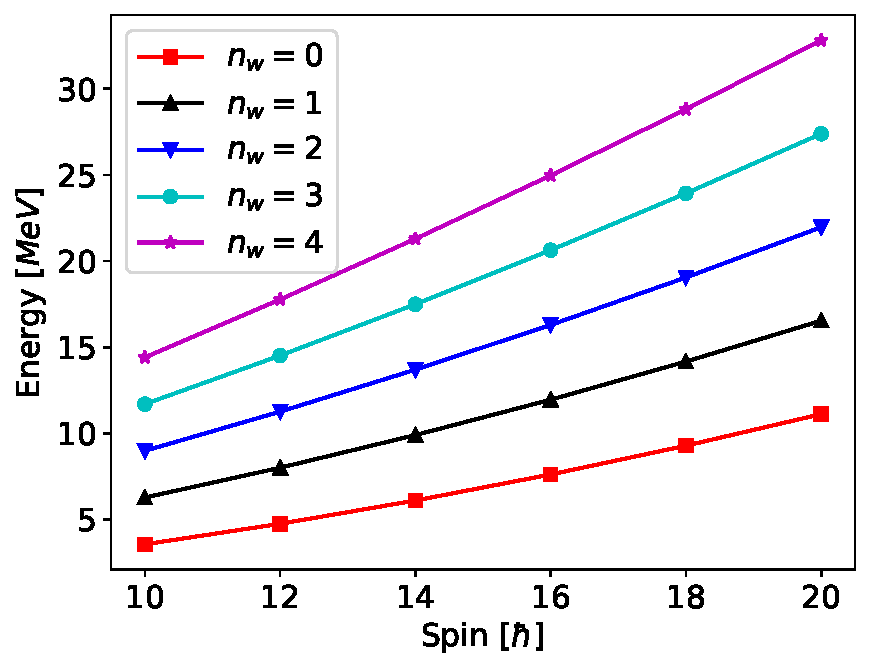
\includegraphics[width=1\linewidth]{figs/simple_wobbling_spectrum.pdf}
  %  \caption{A family of wobbling bands for a triaxial rigid rotor (schematic representation). The calculations were done for $\mathcal{I}_1:\mathcal{I}_2:\mathcal{I}_3=25:5:2$.}
    % \label{simple-wobbling-family}
\end{minipage}%
\begin{minipage}{.4\textwidth}
  \centering
 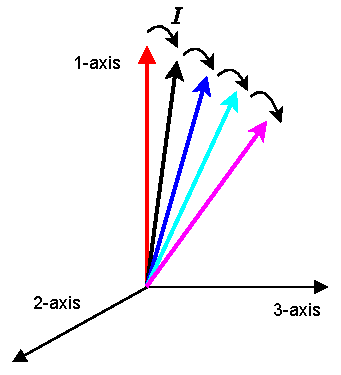
\includegraphics[width=0.8\linewidth]{figs/wobbling_tilting_axis.pdf}
   % \caption{Tilting of the angular momentum away from the rotational axis, with increase in the wobbling phonon excitation.}
    % \label{wobbling-tilt}
\end{minipage}
\label{simple-wobbling-family}
\caption{Family of wobbling bands for a simple triaxial rotor (left-side). Tilting of the angular momentum vector away from the rotational axis with an increase in spin (right-side). This schematic representation was done for an arbitrary set of MOIs $\mathcal{I}_1:\mathcal{I}_2:\mathcal{I}_3=25:5:2$.}
\end{figure}

It is important to mention that the wobbling spectrum described by Eq. \ref{wobbling_eq} and graphically represented in Figure \ref{simple-wobbling-family} was firstly predicted for an even-even triaxial nucleus \cite{bohr1998nuclear}. This predicted wobbling mode has not been experimentally confirmed yet. However, the first experimental evidence for wobbling excitations in nuclei was for an even-odd nucleus, namely $^{163}$Lu, where a single one-phonon wobbling band was measured initially \cite{odegaard2001evidence}, followed by two additional wobbling bands discovered one year later \cite{jensen2002evidence,jensen2002wobbling}.

After the first discovery of wobbling bands in $^{163}$Lu ($Z=71$), an entire series of even-odd isotopes with $A\approx160$ were experimentally confirmed as \emph{wobblers}: $^{161}$Lu, $^{165}$Lu, $^{167}$Lu, and $^{167}$Ta. In these nuclei, the wobbling mode appears due to the coupling of a valence nucleon (the so-called $\pi(i_{13/2})$ intruder) to a triaxial core, driving the entire nuclear system up to large deformation ($\epsilon\approx0.4$) \cite{schnack1995superdeformed}.

With time, several nuclei in which WM occurs were also reported in regions of smaller $A$. Indeed, two isotopes with $A\approx130$: $^{133}$La \cite{biswas2019longitudinal} and $^{135}$Pr \cite{matta2017transverse,sensharma2019two} were identified as having wobbling bands, which emerged from the coupling with a triaxial even-even core of another intruder (the $\pi(h_{11/2})$ nucleon) for $^{135}$Pr, and an additional pair of positive parity quasi-protons which are making an alignment with the short axis of the triaxial rotor for $^{105}$Pd. The resulting coupling in both cases have a deformation $\epsilon=0.16$ \cite{matta2017transverse,biswas2019longitudinal}, which is smaller than the deformation in the heavier nuclei within the $A\approx160$ region. A third nucleus that also lies in this mass region was confirmed very recently by Chakraborty et. al. in \cite{chakraborty2020multiphonon}, namely the odd-$A$ $^{127}$Xe, where a total of four wobbling bands have been reported by the team (two yrast bands, and two excited phonon bands with $n_w=1$ and $n_w=2$).

Some additional progress towards a more comprehensive wobbling spectroscopy was made in the $A\approx100$ mass region, with experimental evidence for $^{105}$Pd that showed two such bands that are built on a $\nu(h_{11/2})$ configuration, the first one so far in which a valence neutron couples to the triaxial core \cite{timar2019experimental}. The resulting configuration drives the nuclear system up to deformation $\epsilon\approx0.26$.

The heaviest nuclei known so far in which WM has been experimentally observed are the isotopes $Z=79$ with $A=183$ \cite{nandi2020first} and $A=187$ \cite{sensharma2020longitudinal}, respectively. However, for the case of $^{187}$Au, there is an ongoing investigation \cite{guo2020risk} whether the two wobbling bands ($n_w=0$ and $n_w=1$) are bands with wobbling character, or if they are of magnetic nature (which would exclude the wobbling phonon interpretation).

Regarding the wobbling motion for the even-even nuclei (behavior that was described above through the schematic representation from Figure \ref{simple-wobbling-family}), the experimental results are very fragmentary, with unclear evidence on such collective behavior in nuclei. However, some embryos of even-even wobblers have been reported in the recent years. For example, the $^{112}$Ru ($Z=44$) nucleus has three wobbling bands \cite{hamilton2010super}, with two of them being excited (one- and two-phonon wobbling bands). Another example is the even-even $^{130}$Ba ($Z=56$) \cite{petrache2019diversity,wang2020two,chen2019transverse}. Indeed, for $^{112}$Ru, the ground band together with the odd and even spin members of the $\gamma$ band were interpreted as zero-(yrast), one-, and two-phonon wobbling bands. Unfortunately, since there are no data concerning the electromagnetic transitions, its wobbling character is still unclear. On the other hand, for the nucleus $^{130}$Ba, from its recent study regarding the band structure \cite{petrache2019diversity}, a pair of bands with even and odd spins were proposed as zero- and one-phonon wobbling bands, respectively. What is worth noting for this case is the fact that these two bands are built on a configuration in which two aligned protons that emerge from the bottom of $h_{j=11/2}$ shell couple with the triaxial core. One remarks the change in nature of the wobbling motion from a purely collective form, but in the presence of two aligned quasiparticles \cite{wang2020two}.

Regarding the interpretation of the wobbling motion which occurs in the nuclei that were mentioned above, it is mandatory to discuss some aspects related to its behavior with the increase in total angular momentum (nuclear spin). It is a long-lasting debate on whether certain nuclei behave as \emph{longitudinal wobblers} (LW) or \emph{transverse wobblers} (TW). The concepts of LW and TW emerged from an extensive study done by Frauendorf et. al. \cite{frauendorf2014transverse} in which the team discussed the possible coupling schemes that a valence nucleon can create with the triaxial core, thus giving rise to two possible scenarios. Based on microscopic calculations using the Quasiparticle Triaxial Rotor (QTR) model, they showed that if the odd valance nucleon aligns its angular momentum vector $\vec{j}$ with the axis of largest MOI, the nuclear system is of longitudinal wobbling character. On the other hand, if the odd nucleon aligns its a.m. vector $\vec{j}$ with an axis perpendicular to the one with the largest MOI, then the nuclear system has a transverse wobbling character. From the microscopic calculations, it was shown that for LW, the wobbling energy $E_\text{wob}$ (see Eq. \ref{wobbling-energy-relative}) has an \emph{increasing} behavior with an increase in spin, while for TW the energy $E_\text{wob}$ \emph{decreases} with spin.

Within the nuclei that were mentioned above, most of them are of TW type, with only $^{133}$La \cite{biswas2019longitudinal}, $^{127}$Xe \cite{chakraborty2020multiphonon}, and $^{183,187}$Au \cite{nandi2020first,sensharma2020longitudinal} being nuclei with LW character. The energy that characterizes the type of wobbling in a nuclear system is the energy of the first excited band (the one-phonon $n_w=1$ wobbling band) relative to the yrast ground band (zero-phonon $n_w=0$ wobbling band):
\begin{align}
    E_\text{wob}=E_{1}(I)-\left(\frac{E_0(I+1)+E_0(I-1)}{2}\right)\ ,
    \label{wobbling-energy-relative}
\end{align}
with 0 and 1 representing the wobbling phonon number $n_w$.

The odd nucleons that couple with the rigid triaxial core will influence the appearance of a particular wobbling regime (LW or TW). In all the wobblers, there is a proton from a certain orbital that is coupling with the core, except for the case of $^{105}$Pd, where the valence nucleon is a neutron. The nature of the odd quasiparticle (i.e., particle or hole) and its "position" in the deformed $j$-shell (i.e., bottom or top) will determine whether its angular momentum $\vec{j}$ will align with the \emph{short} ($s$) or \emph{long} ($l$) axes of the triaxial rotor, respectively (with the notations short $s$, long $l$, and medium $m$ axes of a triaxial ellipsoid). The reasoning behind this has to do with the minimization of the overall energy of the system: in the first case, a maximal overlap of its density distribution with the triaxial core will determine a minimal energy, while in the second case, a minimal overlap of the density distribution of the particle with the core will result in a minimal energy. Moreover, if the quasiparticle emerges from the middle of the $j$-shell, then it tends to align its angular momentum vector $\vec{j}$ with the \emph{medium} ($m$) axis of the triaxial core. Figure \ref{quasiparticle-alignment} aims at depicting the type of alignment of a quasiparticle with the triaxial core.

\begin{figure}
    \centering
    % 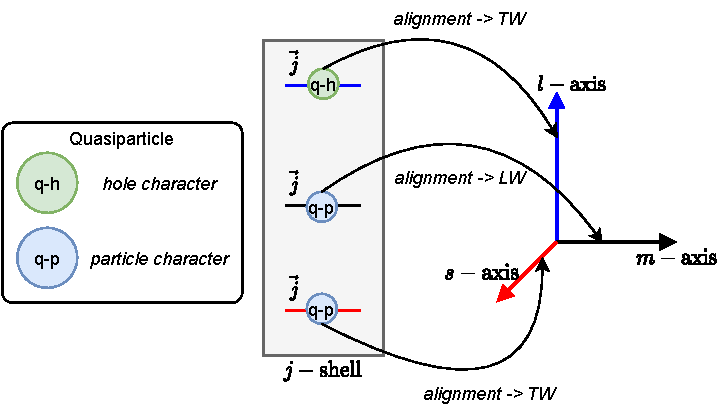
\includegraphics[width=0.85\textwidth]{figs/wobbling_Regimes.pdf}
    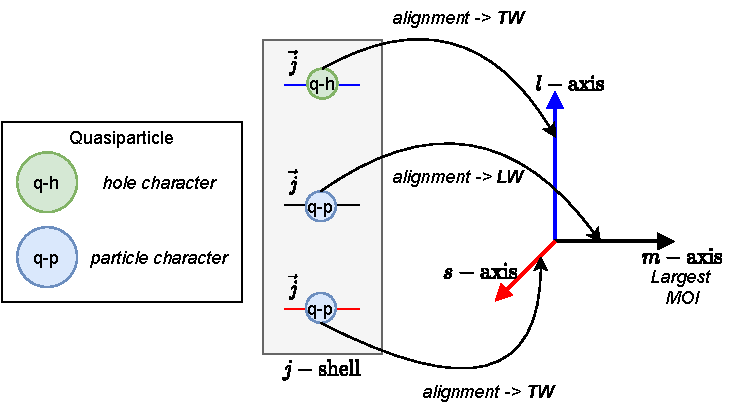
\includegraphics[scale=0.9]{figs/wobbling_Regimes_updated.pdf}
    \caption{The wobbling regimes, Longitudinal Wobbling (LW) or Transverse Wobbling (TW), based on the type of alignment that an odd quasiparticle makes with the principal axes of a triaxial core. Each case depicts a coupling with an odd quasiparticle which emerges from the bottom/middle/top of a $j$-shell. Figure is based on the analysis done in \cite{frauendorf2014transverse}.}
    \label{quasiparticle-alignment}
\end{figure}

As previously mentioned, for a given angular momentum, uniform rotation around the axis with the largest MOI corresponds to minimum energy. For a triaxial rotor emerging from a Liquid Drop, this is equivalent to rotation around the $m$ axis. Therefore, Frauendorf \cite{frauendorf2014transverse} classified the LW as the situation when the odd nucleon will align its angular momentum along the $m$-axis, while TW being the situation where $j$ is aligned perpendicular to the $m$-axis (with $s$- or $l$-axis alignment depending on the $j$-shell orbital from which the odd nucleon arises). It is worthwhile to mention the fact that the analysis done in Ref. \cite{frauendorf2014transverse} was within a so-called \emph{Frozen Alignment} approximation, where the angular momentum of the odd particle $\vec{j}$ is rigidly aligned with one of the three principal axes of the triaxial ellipsoid (that is $s$-, $l$- or $m$-axis).

For a better understanding of the wobbling regimes in terms of angular momentum alignment, the schematic illustration from Figure \ref{wobbling-coupling-scheme} depicts three particular cases, namely a simple wobbler (the case firstly developed by Bohr and Mottelson \cite{bohr1998nuclear}) - shown in inset A.0, a longitudinal wobbler - shown in inset A.1, and lastly a transverse wobbler - shown in inset A.1.

\begin{figure}
    \centering
    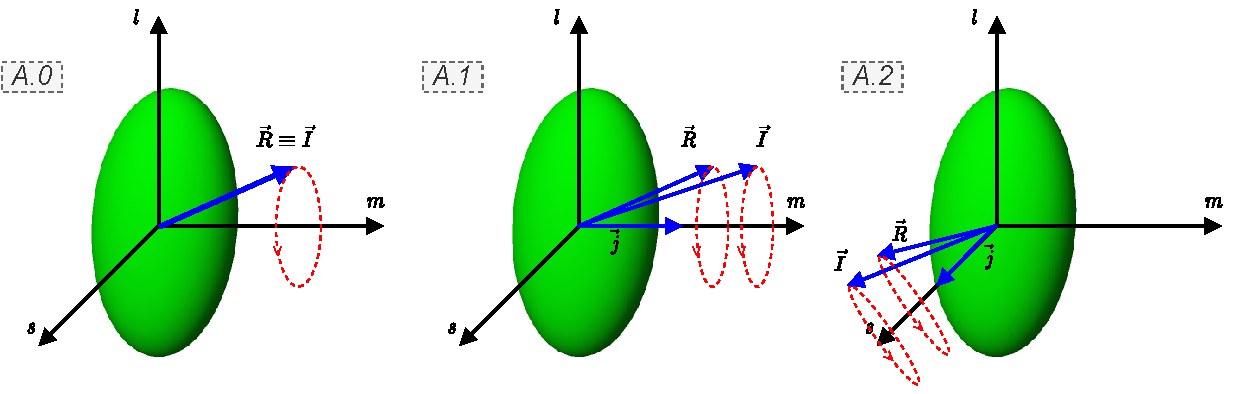
\includegraphics[width=0.95\textwidth]{figs/wobbling_Regimes_COUPLING_SCHEME.pdf}
    \caption{A.0: The geometry for the angular momentum of a simple wobbler. A.1: coupling geometry for a longitudinal wobbler (LW). A.2: coupling geometry for a transverse wobbler (TW). The short-$s$, long-$l$, and medium-$m$ axes are defined in the body-fixed frame. The vectors $\vec{R}$, $\vec{j}$, and $\vec{I}$ represent the set of angular momenta of the core, odd particle, and the total nuclear system, respectively.}
    \label{wobbling-coupling-scheme}
\end{figure}

In terms of its theoretical analysis, the wobbling motion has been studied using multiple models and interpretations. The Triaxial Particle Rotor Model has been widely used over the recent years \cite{bohr1998nuclear,hamamoto2002wobbling,frauendorf2014transverse,tanabe2006algebraic,wen2015wobbling}, these being quantal models that can be exactly solved in the laboratory frame. TRM was, however, firstly introduced for the motion of a rotating nuclear system by Davydov and Filippov in \cite{davydov1958rotational}, where they obtained a complete quantal description for the motion of a triaxial nucleus (because the nucleus must have a well-defined potential minimum at a non-zero value for the triaxiality parameter $\gamma$). Starting from the framework of Cranking Mean Field Theory (CMFT), there were attempts at extending the cranking model for the study of WM. However, using the mean-field approximations, CMFT only helps at describing the yrast sequence for a given configuration. To improve that, the framework was extended with proper quantum correlations by incorporating the Random Phase Approximation (RPA) theory (see Refs. \cite{shimizu1995nuclear,matsuzaki2002wobbling,matsuzaki2003dynamical,matsuzaki2004instability,matsuzaki2004nuclear,shimizu2005high,shimizu2008parametrizations,shoji2009microscopic} for more details).  The method of Collective Hamiltonian \cite{chen2014collective,chen2016wobbling} was used for the investigation of wobbling spectra in nuclei with the help of deformed potentials which were calculated from the Tilted Axis Cranking (TAC) model. TAC single $j$-shell model is also used for the description of the chiral vibrations and rotational motion in deformed nuclei \cite{mukhopadhyay2007chiral,qi2009chirality}. Mean-field approximations were also developed by the so-called \emph{generator coordinate method after angular momentum projection} (GCM+AMP for short), with calculations that emerged from intrinsic cranking states \cite{oi2000wobbling}. Some analytical solutions were also developed (based on certain approximations), such as the harmonic approximation (HA) \cite{bohr1998nuclear,frauendorf2014transverse,chen2014collective,raduta2017semiclassical}, Dyson boson expansion \cite{raduta2017semiclassical,raduta2020new}, and Holstein-Primakoff (HP) formula \cite{tanabe1971triaxiality,tanabe2006algebraic,tanabe2008selection,raduta2017semiclassical,raduta2020new}. The angular momentum projections were also incorporated into the mean-field framework, with the recent development of a completely microscopic description of the wobbling motion by Shimada et. al. \cite{shimada2018rotational}. A Projected Shell Model (PSM) \cite{hara1995projected} which starts from the shell-model configuration mixing that is based on a Nilsson deformed mean field was also used for the theoretical study concerning WM. There are alternative developments based on the PSM approach, based on Density Functional Theories (DFT) that can be both non-relativistic \cite{zhao2016configuration} as well as relativistic \cite{konieczka2018gamow}.

Other tools that proved to be very efficient for the analysis of the wobbling nuclei are the semi-classical approaches, through which one can obtain equations of motion that describe the nuclear system quite well, starting from quantal Hamiltonians and further applying some de-quantization procedures. The semi-classical approach applied to generalized rotor Hamiltonians has the \emph{advantage} of keeping close contact with the classical picture embedded in the dynamic of the systems. Recently, there has been quite an impressive progress towards realistic description of the wobbling motion \cite{raduta2007semiclassical,frauendorf2014transverse,raduta2017semiclassical,raduta2018wobbling,budaca2018tilted,raduta2020approach,raduta2020towards}. As a matter of fact, the present team was able to describe (with a very good agreement) the experimental data concerning the wobbling energies and electromagnetic (e.m.) transition probabilities for the Lu isotopes with $A=161,163,165,167$ (see the work done in Refs. \cite{raduta2017semiclassical,raduta2018wobbling}), and more recently the odd-$A$ $^{135}$Pr isotope \cite{raduta2020new}. Indeed, starting from a quantal Hamiltonian specific to a triaxial rotor model (that is a triaxial core coupled with an odd valence nucleon) and applying the Time-Dependent Variational Equation (TDVE), with a trial function that was carefully chosen, the complete wobbling spectrum of the mentioned isotopes was reproduced, together with the e.m. (intra-band and inter-band) transitions.

Concluding this section, the importance of nuclear triaxiality and the challenges of identifying it experimentally were contoured in the beginning, serving as the starting point of the current work. 
Going further, the structure of this  work is as follows. In Section 2, an overview with regards to the team's previous reinterpretation of the wobbling band structure in $^{163}$Lu will be illustrated. This will be the \emph{core-idea} that serves as the foundation of this newly developed model. The theoretical formalisms and analytical formulas will be  presented in Section 3. Experimental results concerning the wobbling spectrum of this isotope will be compared with the newly obtained data in Section 4. Overall conclusions and discussions are reserved for Section 5.
% \section{Re-interpretation of the wobbling bands structure for $^{163}$Lu}
\section{\texorpdfstring{Re-interpretation of the wobbling bands in $^{163}$Lu}%
                               {Re-interpretation of the wobbling bands structure for 163Lu}}

Now, it is worth mentioning the latest progress made by the present team towards the actual interpretation of the wobbling structure of $^{163}$Lu. Considered the \emph{best wobbler} to date, $^{163}$Lu has a rich wobbling spectrum \cite{odegaard2001evidence,jensen2002evidence}, with no less than four such wobbling bands: one yrast - $TSD_1$, which has a zero-phonon wobbling number $n_w=0$), and three excited wobbling bands - $TSD_{2,3,4}$ with their corresponding wobbling phonon numbers $n_w=1,2,3$, respectively. The name TSD comes from Triaxial Strongly Deformed bands. The triaxial bands emerge due to the coupling of an odd-$\vec{j}$ nucleon with an even-even triaxial core. Thus, for $^{163}$Lu, it is the intruder $\pi(i_{13/2})$ that couples to the triaxial core \cite{odegaard2001evidence,hamamoto2002wobbling,jensen2002wobbling}, driving the nuclear system up to large deformation, and stabilizing the deformed structure. Indeed, a triaxial shape with deformation parameters $(\epsilon_2,\gamma)\approx(0.38,+20^\circ)$ is assumed to be in agreement with the observed data, based on calculations using the Ultimate Cranker Code \cite{bengtsson1990high} for the potential energy surface (PES).

In terms of experimental evidence which should be pointing out wobbling nature for the four TSD bands belonging to $^{163}$Lu, the large transition quadrupole moment $Q_t \approx 10\ b$ \cite{gorgen2004quadrupole} (which is substantially larger than it is the case for normal-deformed bands), the predominantly $E2$ character of the transitions linking adjacent bands ($I\to I-1$), a large $E2/M1$ mixing ratio $\delta>1$ for the transitions linking the yrare ($n_w=1$) and yrast ($n_w=0$) bands (which obviously should result in smaller transitions with magnetic character, or in other words, there is no $M1$ dominance) are clear fingerprints of wobbling nature. For a set of results concerning these quantities (both theoretical and experimental), see Ref. \cite{raduta2017semiclassical}, and the references cited therein. Another quantity that indicates strong deformation with wobbling character is the relative rigid rotor energy, and for this isotope, calculations show that all four bands have similar behavior with respect to this value (see Figures 3 and 4 from Ref. \cite{hagemann2005triaxiality}).

Considering the experimental evidence which was indicated above and calculations based on particle rotor models, it can be summarized that the \emph{generally accepted} formalism for the band structure in $^{163}$Lu is the following:
\begin{itemize}
    \item There are three excited wobbling bands (w.b.): $TSD_2$, $TSD_3$, and $TSD_4$.
    \item The three excited w.b. have wobbling-phonon numbers $n_{w_2}=1$, $n_{w_3}=2$, and $n_{w_4}=3$, respectively.
    \item All three bands are built on top of the yrast state (the ground state band) with zero-wobbling-phonon number $n_{w_1}=0$.
    \item Stable triaxial super-deformation is achieved due to the alignment of the odd $\pi(i_{13/2})$ nucleon which couples to a triaxially deformed core $\vec{R}$.
    \item $TSD_{1,2,3}$ have all positive parity $\pi_1=\pi_2=\pi_3=+1$, while the spin states belonging to $TSD_4$ have negative parity $\pi_4=-1$. All states within the four bands have a half-integer spin.
 \end{itemize}

In accordance with the band structure which was just formulated, a full description of the wobbling spectrum of $^{163}$Lu was done within a semi-classical formalism by Raduta et. al. \cite{raduta2017semiclassical}. Therein, with the TDVE applied on the PRM Hamiltonian with a trial wave-function that encapsulates both the states of the deformed nucleus $I$ and the single-particle states $j$, a set of analytical expressions for the excitation energies of all four bands was obtained. The energies belonging to the excited wobbling phonons were populated by the action of a phonon operator $\Gamma^\dagger$ on the ground state. Indeed, by acting with the phonon operator on the ground state with the spin $I=R+j$ and $R=0,2,4,\dots$, the states from $TSD_2$ ($n_w=1$) can be obtained. By applying twice ($n_w=2$) the phonon operator, the rotational states from $TSD_3$ will be created. Lastly, the states from $TSD_4$ are obtained with the action on the ground state with three ($n_w=3$) phonon operators: two of positive parity and one of negative parity (due to the overall negative parity $\pi_4=-1$ of $TSD_4$). One has to remark the fact that for $TSD_4$, the model assumes an odd-particle-rotor with a different intruder: the $\pi(h_{9/2})$ nucleon. This was suggested by the negative parity orbital which might be occupied by this proton, in the spherical shell model. Several calculations in the literature point out that this nucleon might be causing the third excited wobbling band to have negative parity \cite{jensen2004coexisting}. It is worthwhile mentioning that for the work described in \cite{raduta2017semiclassical}, the variational principle was only applied for the states in $TSD_1$ since the other three wobbling bands are obtained through phononic excitations with the corresponding operator.

In what follows, it is useful to introduce some notations that will refer to the formalisms developed by the team in describing the wobbling motion in $^{163}$Lu. As such, the work developed in \cite{raduta2020approach,raduta2020towards} will be denoted to \texttt{W1}, while the current work (which is in fact an extension of \texttt{W1}) will be shortly denoted by \texttt{W2}. For the sake of a self-consistent presentation, in the following subsection \ref{subsection:w1} a brief overview of the recently published work \texttt{W1} will be made, with further development that has \texttt{W1} as a starting ground being presented in the second subsection \ref{subsection:w2} - representing the \emph{core concept} of the current team's investigation.

\subsection{\texttt{W1} - Signature Partner Bands}
\label{subsection:w1}

Working with a semi-classical approach that is based on the triaxial particle rotor model, a full description of the wobbling bands for $^{163}$Lu was achieved, but with a slightly modified band structure. Indeed, rather than applying a TDVE just for the yrast $TSD_1$ band, the states from $TSD_2$ were also obtained variationally. This was possible due to the different coupling schemes that emerged for $TSD_1$ and $TSD_2$, respectively. More precisely, in \cite{raduta2020towards} and \cite{raduta2020approach} there are three different coupling schemes $(\vec{R}+\vec{j})$: states from $TSD_1$ arise from the odd $\pi(i_{13/2})$ intruder coupling with a core with angular momentum sequence $R_1=0,2,4,\dots$; states from $TSD_2$ arise from the same odd proton but coupling with a different triaxial core with angular momentum sequence $R_2=1,3,5,\dots$. The band $TSD_3$ is obtained as a set of states which are built on top of $TSD_2$, with the action of a wobbling frequency with wobbling phonon number $n_w=1$; this being different than the band structure previously mentioned were the third band was a two-phonon excitation of the yrast $TSD_1$. Lastly, the fourth band $TSD_4$ is a ground state band which results from the coupling of the same core as for $TSD_2$ (that is defined with the angular momentum sequence $R_2=1,3,5,\dots$) but with a different odd nucleon: $\pi(h_{9/2})$. Consequently, $TSD_2$ and $TSD_4$ are yrast states, alongside $TSD_1$. Each band represents a collection of energy levels describing ground states that correspond to distinct sets of angular momenta.

For the first three bands, the MOIs are the same, and they are considered to be free parameters within the numerical calculations. However, this is not true for the fourth band, where a different set of MOIs had to be introduced, since for $TSD_4$ the core polarization effects are changed by coupling scheme.

Using \texttt{W1}, the final results pointed out to a largest MOI corresponding to the 1-axis (with $\mathcal{I}_1$ being the largest MOI obtained through the fitting procedure), making the system rotate around the 1-axis (that is the short axis). Moreover, the odd proton is aligned to the short axis as well, suggesting that the nucleus has an LW character. By representing the experimental wobbling energies according to Eq. \ref{wobbling-energy-relative}, it was obtained that both theoretical, as well as the experimental values, were increasing functions with respect to an increase in angular momentum (keep in mind that the first wobbling band $n_w=1$ within the \texttt{W1} model is $TSD_3$). The agreement between the two sets of data (see Figure 6 from \cite{raduta2020approach}) indicates that the condition for LW/TW character of the wobbling bands stated by Frauendorf et. al. in \cite{frauendorf2014transverse} is not strictly related to the increasing/decreasing wobbling energy $E_\text{wob}$. In fact, Guo et. al. \cite{guo2020risk} also point out that the approximation of Frozen Alignment (FA) from \cite{frauendorf2014transverse} neglects the Coriolis interaction of the single-particle. There is an ongoing debate whether the behavior of an LW or TW triaxial nucleus is strictly related to the change in $E_{wob}$ with total a.m. \cite{tanabe2017stability,frauendorf2018comment,tanabe2018reply}.


A final aspect that needs to be mentioned regarding \texttt{W1} has to do with the interpretation of $TSD_1$ and $TSD_2$ as being Signature Partner Bands (SPB). Signature \cite{bohr1998nuclear} is a quantum property that appears in deformed systems. It is strictly related to the invariance of a system with quadrupole deformation to a rotation by an angle $\pi$ around a principal axis. For example, a rotation around the $x$-axis will be defined as an operator:
\begin{align}
    \hat{R}_x=e^{i\pi\hat{I}_x}\ .
\end{align}

As for the framework used in \cite{raduta2020approach,raduta2020towards}, due to the wave-function describing the system being written as a product between the $\ket{I}$ basis state corresponding to the total angular momentum and the single-particle basis state $\ket{j}$, the rotation operator used in \texttt{W1} achieves the following form:
\begin{align}
    \hat{R}_x(\pi)=e^{-i\pi\hat{I}_x}\otimes e^{-i\pi\hat{j}_x}\ .
\end{align}

If the system has axial symmetry, only the rotation around any of the principal axes that are perpendicular to the symmetry one can define the signature quantum number. Consequently, the signature is a property specific to a deformed system and it translates to a so-called \emph{deformation invariance} with respect to space and time reflection properties \cite{bohr1998nuclear}. For an even-even nucleus, the signature operator $\hat{R}_x$ has two eigenvalues, -1 and 1. For the even-odd case, the eigenvalues are $-i$ and $+i$, and depending on its total spin, the signatures can have two values, given by the following assignment:
\begin{align}
    \alpha_I=\frac{1}{2}\left(-1\right)^{I-1/2}\ .
    \label{signature-formula-odd-nuclei}
\end{align}

Indeed, Eq. \ref{signature-formula-odd-nuclei} describes the signature quantum number for a state of angular momentum $I$ belonging to an odd mass nucleus. Such a rotational band with a sequence of states differing in spin by $\Delta I=1$ will be divided into two branches, each branch consisting of levels differing in spin by $\Delta I=2$, being related by the signature number $\alpha_I=\pm 1/2$. In \cite{raduta2020approach} the signature concept is brought to the classical picture associated with a triaxial nucleus employing rotation operators which act on the trial function (this function is a product of two coherent states, one that is associated to the core and one to the valence nucleon). Eqs. 27-29 from \cite{raduta2020approach} will extract two signatures for $TSD_1$ and $TSD_2$, namely the \emph{favored} signature $\alpha_{1f}=+1/2$ for the first band, and \emph{un-favored} signature $\alpha_{2u}=-1/2$ for the second band, respectively. A justification for the possibility of $TSD_1$ and $TSD_2$ of being SPB was based on the calculation of the triaxial potential (which was systematically performed in \cite{raduta2017semiclassical} and \cite{raduta2018wobbling}), concluding that the minimum is very deep, preventing in this way the states from $TSD_2$ to share other minima through tunneling effects. Other experimental and theoretical results \cite{sun1994varied,khalaf11properties,uma2015deltai,mittal2016signature} for deformed nuclei around this mass region suggest that the calculations performed in \texttt{W1} regarding the connection between $TSD_1$ and $TSD_2$ as belonging to a signature splitting phenomenon are valid and consistent with already existing interpretations.

It is instructive to mention a few key-points which arise based on the above discussion regarding \texttt{W1}:

\begin{enumerate}[(a)]
    \item The wobbling band structure in $^{163}$Lu was re-interpreted: three bands are now yrast ground states, and only $TSD_3$ is one-phonon excited wobbling band (built on top of $TSD_2$)
    \item Both $TSD_1$ and $TSD_2$ are obtained variationally, by solving the time dependent variational equation associated to the initial quantal Hamiltonian
    \item There are three different $R+j$ coupling schemes that will produce the entire spectra:
    \begin{enumerate}[(i)]
        \item Coupling $C_1$: The odd proton $j_1={13/2}$ is coupled to a core sequence with a.m. $R_1=0,2,4,\dots$ (even spin states for the triaxial rotor).
        \item Coupling $C_2$: The same odd proton $j_1={13/2}$ as in $C_1$ is coupled to a core sequence with a.m. $R_2=1,3,5,\dots$ (odd spin states for the triaxial rotor).
        \item Coupling $C_3$: A different odd proton $j_2={9/2}$ is coupled to the same core as in $C_2$.
    \end{enumerate}
    \item Two different sets of MOIs corresponding to the triaxial nucleus (that is the rotor coupled with the odd proton) are obtained as fitting parameters throughout the numerical calculations: one for the set $TSD_{1,2,3}$ and one for $TSD_4$.
    \item $TSD_1$ and $TSD_2$ are Signature Partner Bands: with $TSD_1$ ($TSD_2$) being the favored (un-favored) partner. Their corresponding signature quantum numbers are $\alpha_{1f}=+1/2$ and $\alpha_{2u}=-1/2$.
    \item As a side-by-side comparison with regards to the overall agreement with the experimental data, \texttt{W1} yielded better results when compared to the previous work depicted in Ref. \cite{raduta2007semiclassical}, although it must be mentioned that both models are based on semi-classical approaches.
\end{enumerate}

A diagram that shows the workflow involved in \texttt{W1} can be seen in Figure \ref{w1-model-worfklow} from the Appendix. Also, a comparison with previous calculations can be seen in Figure 21 from Ref. \cite{raduta2020approach}.

\subsection{\texttt{W2} - Signature Partner Bands + Parity Partner Bands}
\label{subsection:w2}

The main question which can be asked regarding the formalism \texttt{W1} that was described in \ref{subsection:w1} is whether it is possible to obtain a \emph{unified} description for all four bands in $^{163}$Lu concerning the coupling scheme. In other words, it is worth investigating the possibility of having a unique single-particle state $j$ that is coupled to a core of positive parity for the bands $TSD_{1,2,3}$ and a core of negative parity for $TSD_4$.

Fortunately, the answer is positive: starting from the semi-classical formalism of \texttt{W1}, one can properly adjust the coupling scheme, making sure that the entire numerical recipe used for obtaining the energy spectrum of $^{163}$Lu remains consistent with the experimental results.

Regarding the unique single-particle that couples to the triaxial core, it is natural to pick the $i_{13/2}$ proton (that is $j$ from \texttt{W1}). The reasoning behind this choice has to do with the microscopic calculations \cite{jensen2002wobbling,hagemann2003quantized,jensen2004coexisting} that showed stable triaxial structures in the $^{163}$Lu potential energy surface when the triaxial core couples with a highly aligned $j$-shell particle, strongly indicating the $\pi(i_{13/2})$ proton. Keep in mind that a highly aligned $j$-nucleon will \emph{prefer} to keep a certain triaxial deformation when coupled to a core \cite{hamamoto1983intrinsic,hamamoto1987rotational,hamamoto2016interplay} (in the sense that the triaxiality parameter $\gamma$ will have a certain value based on the orbital of the odd nucleon), and using microscopic calculations following the Ultimate Cranker code, it has been shown that a value of $\gamma\approx+20^\circ$ is preferred by the odd $\pi(i_{13/2})$ nucleon.

By taking $j_1$ as the sole intruder that couples to a positive core and also a negative core, the sequences with even/odd integer spins for the core do not change. In fact, the coupling schemes can be readily obtained, making sure that the final (experimental) spin sequences for each TSD band are intact. 

\begin{enumerate}[(a)]
    \item Coupling $C'_1$: the odd $j$ proton aligns with the core of even-integer spin sequence $R_1=0,2,4,\dots$, with a parity of the $R_1$ core that is positive $\pi(R_1)=+1$.
    \item Coupling $C'_2$: the odd $j$ proton aligns with the core of even-integer spin sequence $R_2^+=1,3,5,\dots$, with a parity of the $R_2^+$ core that is positive $\pi(R_2^+)=+1$.
    \item Coupling $C'_3$: the odd $j$ proton aligns with the core with an odd-integer spin sequence $R_2^-=1,3,5,\dots$, which has negative parity $\pi(R_2^-)=-1$.
\end{enumerate}

From the three schemes defined above, it is clear that $C'_1$ corresponds to the yrast $TSD_1$, $C'_2$ to the ground state $TSD_2$, and finally $C'_3$ to the ground state $TSD_4$. Obviously, the odd valence nucleon $j$ has a positive parity $\pi_{j}=+1$. There has not been attributed a coupling scheme for $TSD_3$, since this band still remains as the one-wobbling phonon excitation that is built on top of $TSD_2$ with the action of a phonon operator which will be characterized later on. The three couplings are schematically represented in Figure \ref{three-couplings}. One should keep in mind the fact that $\vec{j}$ is aligned with the axis with the largest MOI does not necessarily mean the fact that the model works within the Frozen Alignment approximation - it is just an illustration.

\begin{figure}
    \centering
    % 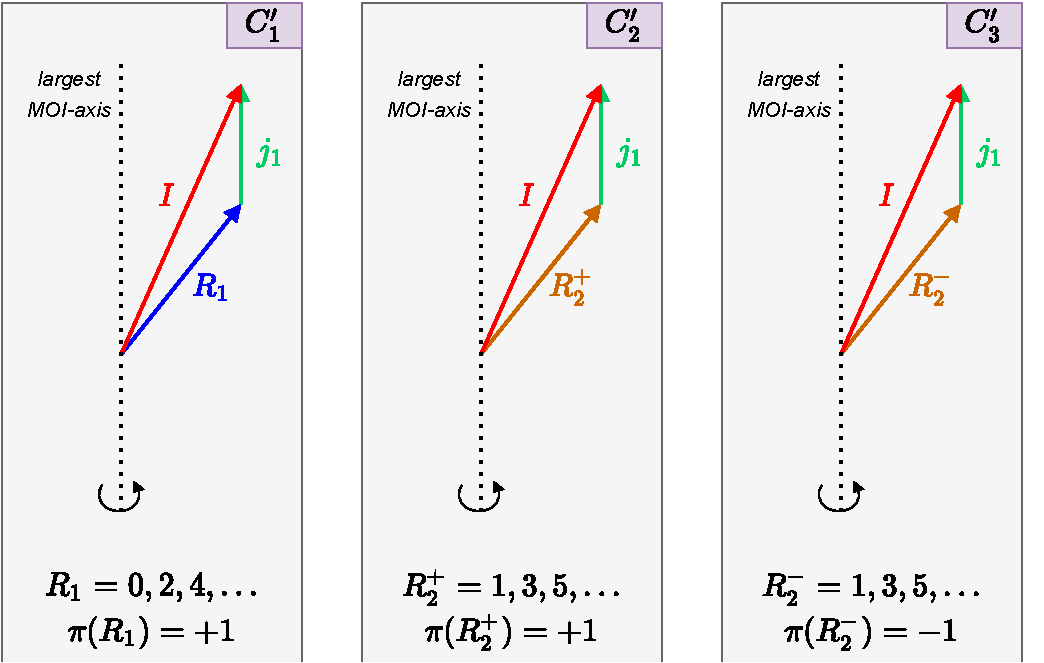
\includegraphics[width=0.95\textwidth]{figs/coupling_schemes_C1C2C3.pdf}
    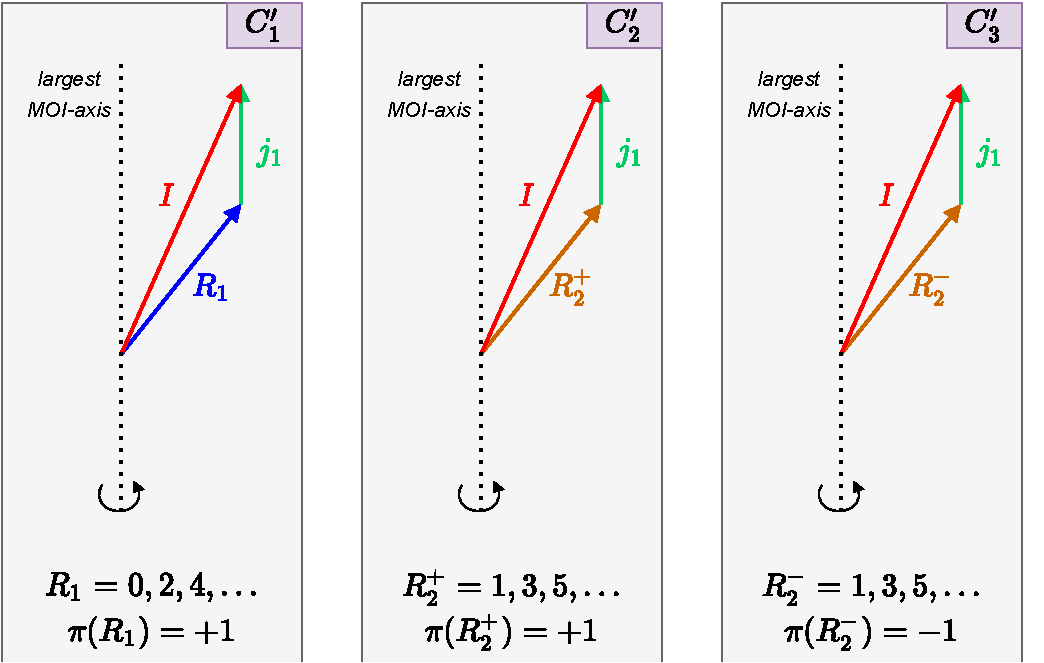
\includegraphics[scale=0.65]{figs/coupling_schemes_C1C2C3.pdf}
    \caption{A schematic representation with the three coupling schemes that characterize the \texttt{W2} model. The same odd particle (the $j_1=i_{13/2}$ proton) is coupled with two positive cores with even/odd integer spin sequences for $TSD_1$/$TSD_2$, and one negative core in the case of $TSD_4$ with odd integer spin sequence. The total spin of the system precesses around the axis with the largest MOI, as it is the case for a triaxial rotor.}
    \label{three-couplings}
\end{figure}

It is expected that the Hamiltonian of the system will keep a similar form since there are no new interactions or modified particle-core states added in the problem. The argument holds because the coupling scheme which involves the fourth triaxial band $TSD_4$ only the single-particle angular momentum state changes, but the core has negative parity. As a result, the treatment of the problem will follow the same line as it did in the \texttt{W1} case.

The last step in searching for an unified coupling scheme in $^{163}$Lu is to establish a possible relationship between the four bands. As per the calculations involved in \texttt{W1}, it was proven that signature is a good quantum number and indeed, a sign that $TSD_1$ and $TSD_2$ are signature partners emerged. Their overall similar properties and spin difference enforce this argument. Furthermore, in this new \texttt{W2} approach, the difference in parity between the $TSD_2$ and $TSD_4$ but the same angular momentum sequence of their corresponding triaxial core $R_2^+$ and $R_2^-$ strongly suggest that the two bands are \emph{Parity Partner Bands}: two rotational sequences with energy states characterized by opposite parity, increasing energy that follows a trend $\propto I(I+1)$, and a spin difference $\Delta I=2$ between states belonging to the same band. In the following section, calculations that will show that parity is indeed a good quantum number for the triaxial rotor + odd-particle system will be provided. For what it is worth mentioning now is that the concept of parity partners between $TSD_2$ and $TSD_4$ emerge from the idea that a stable strongly deformed structure is achieved from a single quasiparticle that moves in a quadrupole mean-field generated by a triaxial even-even core. However, there is a splitting in two different cases of coupling mechanisms, namely $C'_2$/$C'_3$ depending on the alignment of the high-$j$-shell particle with a core of positive/negative parity.

Similar structures with alternating positive-negative parity bands have been also reported in other nuclei such as $^{40}$Ca \cite{torilov2004spectroscopy}, or some heavier isotopes like $^{218}$Fr \cite{debray2000alternating}. In fact, one of the authors of this present work developed an unified description of states with positive and negative parity in odd-mass nuclei \cite{radutaa2009csm,raduta2011simultaneous}, although therein, a quadrupole-octupole term was introduced within the particle-core Hamiltonian to describe this feature. Concluding the current subsection, a diagram which shows the workflow involved in \texttt{W2} can be seen in the Figure \ref{w2-model-worfklow} from the Appendix.

\section{Theoretical Background}

In this section, a description of the framework used for obtaining the wobbling spectrum of $^{163}$Lu is made. As stated in the previous section, the system is described with a similar Hamiltonian used in \texttt{W1}, namely the Hamiltonian for the triaxial PRM.
\begin{align}
    H=H_\text{core}+H_\text{s.p.}\ .
    \label{prm-hamiltonian}
\end{align}

The Hamiltonian in Eq. \ref{prm-hamiltonian} describes a system in which an odd $j$ particle interacts with a triaxial even-even core i.e., the odd nucleon is moving in a quadrupole deformed mean-field that is generated by the core. As such, the first $H_\text{core}$ term in the Hamiltonian describes the motion of a triaxial core, while the second term $H_\text{s.p.}$ represents the  valence proton ($j_1$ in this case).

Indeed, the core Hamiltonian is given by:
\begin{align}
    H_\text{core}=\sum_{i=1,2,3}\frac{1}{2\mathcal{I}_i}(I_i-j_i)^2\ ,
    \label{core-hamiltonian}
\end{align}
where the core angular momentum is $\vec{R}=\vec{I}-\vec{j}$ and the terms $\mathcal{I}_i$ represent the moments of inertia for triaxial ellipsoid, along the principal axes. These three moments of inertia will be considered as free parameters in the present calculations, but, compared to the work \texttt{W1}, a unique set of MOIs will be attributed to the four bands, since the triaxial core will create an alignment with a unique single particle, that is $j$. Because of this, there is no option for their nature (i.e., rigid or hydrodynamic).

The single-particle Hamiltonian from Eq. \ref{prm-hamiltonian} is derived from the well-known Nilsson potential \cite{meyer1975collective,wang2008description}:
\begin{align}
    h(\beta_2,\gamma)=C\left\{\cos\gamma Y_{20}(\theta,\varphi)+\frac{\sin\gamma}{\sqrt{2}}\left[Y_{22}(\theta,\varphi)+Y_{2-2}(\theta,\varphi)\right]\right\}\ ,
    \label{nilsson-potential}
\end{align}
where the coupling parameter $C$ causes the level splitting in the deformed field and it is proportional to the quadrupole deformation $\beta_2$. The potential $h$ from Eq. \ref{nilsson-potential} is written in terms of the quadrupole deformation and triaxiality parameter that play the role of deformation parameters within a triaxial system $(\beta_2,\gamma)$. Its expression using the coupling parameter $C$ is widely used when working with a particle-rotor-model \cite{peng2003description,koike2004chiral,wang2007doublet}. For this case, by applying a Wigner-Eckart theorem for the single-j particle, the following expression for $H_\text{s.p.}$ will be obtained:
\begin{align}
    H_\text{s.p.}=\frac{V}{j(j+1)}\left[\cos\gamma(3j_3^2-\vec{j}^2)-\sqrt{3}\sin\gamma(j_1^2-j_2^2)\right]+\epsilon_j\ .
    \label{single-particle-hamiltonian}
\end{align}

This term describes the motion of an odd particle with angular momentum $j$ in a mean-field generated by a triaxial core, with a potential strength $V$ characterized by the quadrupole deformation ($V\propto\beta_2)$. In fact, the single-particle potential strength $V$ will be considered as the fourth free parameter within the calculations and its behavior will dictate the coupling of the $j$ particle with all four TSD bands. The term $\epsilon_j$ from Eq. \ref{single-particle-hamiltonian} represents the single-particle energy that corresponds to the odd $j$ proton from the $i$-orbital.

Regarding the triaxial deformation $\gamma$ which enters in Eq. \ref{single-particle-hamiltonian}, its value will be considered as another free parameter of the current problem. In other words, having $V$ and $\gamma$ as free parameters means that the system will be described by its deformation parameters which will be obtained through a fitting procedure, keeping an agreement with the experimental data regarding the excitation energies of the rotational states belonging to $TSD_{1,2,3,4}$.

From Eqs. \ref{core-hamiltonian} and \ref{single-particle-hamiltonian}, the free parameter set can be obtained, hereafter denoted by $\mathcal{P}$. It comprises three moments of inertia, the single particle potential strength, and the triaxial deformation. As such, $\mathcal{P}$ can be written as:
\begin{align}
    \mathcal{P}=\left[\mathcal{I}_1,\mathcal{I}_2,\mathcal{I}_3,V,\gamma\right]\ .
    \label{parameter-set}
\end{align}

Solving the problem of \texttt{W2} is equivalent to finding the eigenvalues of $H$ given in Eq. \ref{prm-hamiltonian}. In a similar approach as in \texttt{W1}, the eigenvalues of interest are obtained on the base of a semi-classical approach. Thus, the first step is to perform a de-quantization procedure on $H$ through a TDVE \cite{raduta2007semiclassical,budaca2018tilted,raduta2017semiclassical}:
\begin{align}
    \delta\int_0^t\bra{\Psi_{IjM}}H-i\frac{\partial}{\partial t'}\ket{\Psi_{IjM}}dt'=0\ .
    \label{tdve}
\end{align}

Working within a semi-classical approach allows one to keep close contact with the system's dynamics in terms of equations of motion for the generalized coordinates. The trial function from Eq. \ref{tdve} is carefully chosen as a product of two basis states comprising the states with total angular momentum $I$ and $j$, respectively:
\begin{align}
    \ket{\Psi_{IjM}}=\mathbf{N}e^{z\hat{I}_-}e^{s\hat{j}_-}\ket{IMI}\ket{jj}\ ,
    \label{trial-function}
\end{align}
where the operators $\hat{I}_-$ and $\hat{j}_-$ denote the lowering operators for the intrinsic angular momenta $\vec{I}$ and $\vec{j}$, respectively, and $\mathbf{N}$ plays the role of the normalization constant. One must remark the fact that the states $\ket{IMI}, \ket{jj}$ from Eq. \ref{trial-function} are extremal states for the operators $(\hat{I}^2,\hat{I}_3)$ and $(\hat{j^2},\hat{j_3})$, respectively, and they correspond to the maximally allowed states for a given set of angular momenta $I$ and $j$. As an observation, the trial function is an admixture of components of definite $K$, which is consistent with the fact that for a triaxial nucleus, $K$ is not a good quantum number.

The variables $z$ and $s$ from Eq. \ref{trial-function} are complex functions of time, and they play the role of classical coordinates in the phase spaces that describe the motion of the core and the odd particle:
\begin{align}
    z=\rho e^{i\varphi}\ ,\ s=fe^{i\psi}\ .
    \label{complex-variable-set}
\end{align}

In order to obtain a set of classical equations in a Hamilton canonicl form, a new pair of variables are introduced: 
\begin{align}
    r=\frac{2I}{1+\rho^2}\ ,\ t=\frac{2j}{1+f^2}\ ,
\end{align}
where $r\in\left[0,2I\right]$ and $t\in\left[0,2j\right]$.Thus the equations of motion acquire the form:
\begin{align}
    \frac{\partial\mathcal{H}}{\partial r}&=\dot{\varphi}\ ;\ \frac{\partial\mathcal{H}}{\partial \varphi}=-\dot{r}\ , \nonumber\\
    \frac{\partial\mathcal{H}}{\partial t}&=\dot{\psi}\ ;\ \frac{\partial\mathcal{H}}{\partial \psi}=-\dot{t}\ .
    \label{eq-motion}
\end{align}

The function $\mathcal{H}$ denotes the average of the Hamiltonian operator $H$ (Eq. \ref{prm-hamiltonian}) with the trial function $\ket{\Psi_{IjM}}$ given in Eq. \ref{trial-function}, and it plays the role of classical energy:
\begin{align}
    \mathcal{H}(\varphi,r;\psi,t)=\bra{\Psi_{IjM}}H\ket{\Psi_{IjM}}\ ,
\end{align}

Starting from the equations of motion given in Eq. \ref{eq-motion}, one can observe that the function $\mathcal{H}$ is a constant of motion, that is $\dot{\mathcal{H}}\equiv0$. This equation will define a surface, a so-called equi-energy surface $\mathcal{H}=\text{const}$. It is worth mentioning the fact that such an equality holds since the entire set of equations of motion emerged from a variational principle. The sign of the Hessian associated to this classical function will indicate its stationary points. Among them, some are minima. We are interested in depicting the minima when the following ordering of MoI's holds: $\mathcal{I}_1>\mathcal{I}_2>\mathcal{I}_3$. There is no restriction on $\gamma$.

With a linearization procedure for the equations of motion around the minimum point  of $\mathcal{H}$, a dispersion equation will be obtained:
\begin{align}
    \Omega^4+B\Omega^2+C=0\ .
    \label{dispersion-eq}
\end{align}

The above equation describes a harmonic type of motion for the nuclear system, with the solutions to this algebraic equation as the \emph{wobbling frequencies} $\Omega$. The terms $B$ and $C$ are  functions of total angular momentum $I$, single particle a.m. $j$, inertial parameters $A_k=1/(2\mathcal{I}_k)\ ,\ k=1,2,3$, single particle potential strength $V$, and triaxiality parameter $\gamma$.  The $B$ term from Eq. \ref{dispersion-eq} has the expression \cite{raduta2020approach}:
\begin{align}
 -B=\left[(2I-1)(A_3-A_1)+2jA_1\right]\left[(2I-1)(A_2-A_1)+2jA_1\right]+8A_2A_3Ij+\text{T}_B^1\text{T}_B^2\ ,
 \label{b_term}
 \end{align}
 where the terms $\text{T}_B^1$ and $\text{T}_B^2$ are defined defined as:
 \begin{align}
 \text{T}_B^1&=\left[(2j-1)(A_3-A_1)+2IA_1+V\frac{2j-1}{j(j+1)}\sqrt{3}(\sqrt{3}\cos\gamma+\sin\gamma)\right]\ , \nonumber \\
 \text{T}_B^2&=\left[(2j-1)(A_2-A_1)+2IA_1+V\frac{2j-1}{j(j+1)}2\sqrt{3}\sin\gamma\right]\ .
 \label{b_term-plus}
\end{align}

Accordingly, the $C$ term from Eq. \ref{dispersion-eq} has the expression \cite{raduta2020approach}:
\begin{align}
    C=&\left\{\left[(2I-1)(A_3-A_1)+2jA_1\right]\text{T}_C^1
- 4IjA_3^2\right \} \nonumber\\
      &\times\left\{\left[(2I-1)(A_2-A_1)+2jA_1\right]\text{T}_C^2-4IjA_2^2\right\}\ ,
      \label{c_term}
\end{align}
where the terms $\text{T}_C^1$ and $\text{T}_C^2$ are defined defined as:
\begin{align}
    \text{T}_C^1&=\left[(2j-1)(A_3-A_1)+2IA_1+V\frac{2j-1}{j(j+1)}\sqrt{3}(\sqrt{3}\cos\gamma+\sin\gamma)\right]\ , \nonumber\\
    \text{T}_C^2&=\left[(2j-1)(A_2-A_1)+2IA_1+V\frac{2j-1}{j(j+1)}2\sqrt{3}\sin\gamma\right]\ . 
    \label{c_term-plus}
\end{align}

It can be seen that the terms which enter in $B$ and $C$, namely $(\text{T}_B^1,\text{T}_B^2)$ from Eq. \ref{b_term-plus} and $(\text{T}_C^1,\text{T}_C^2)$ from Eq. \ref{c_term-plus} that enter in $B$ and $C$ correspond to the quadrupole deformation that causes the single-particle to move in the mean-field of the triaxial core. The terms also define the triaxiality that the nucleus achieves once the odd proton couples to the triaxial core, driving the system up to a large (and stable) deformation.

Going back to Eq. \ref{dispersion-eq}, under the restrictions for the MOIs defined above, the dispersion equation admits two real and positive solutions (hereafter denoted with $\Omega_1^I$ and $\Omega_2^I$, where $\Omega_1^I<\Omega_2^I$) defined for $j_1=i_{13/2}$, given by:
\begin{align}
    \Omega_{1,2}^I=\sqrt{\frac{1}{2}\left(-B\mp(B^2-4C)^{1/2}\right)}\ .
    \label{wobbling-frequencies}
\end{align}

These two solutions are interpreted as \emph{wobbling frequencies} associated with the motion of the core, and the motion of the odd-particle. As such, each wobbling frequency has an associated wobbling-phonon number:
\begin{align}
    \Omega_1^I \to n_{w_1}\ ;\ \Omega_2^I \to n_{w_2}\ .
\end{align}


Now  the analytical expressions for the four TSD bands in $^{163}$Lu are readily obtained:
\begin{align}
    E_\text{TSD1}^I&=\epsilon_j+\mathcal{H}_\text{min}^{(I,j)}+\mathcal{F}_{00}^I\ ,\ I=13/2,17/2,21/2\dots \nonumber \\
    E_\text{TSD2}^I&=\epsilon_j^1+\mathcal{H}_\text{min}^{(I,j)}+\mathcal{F}_{00}^I\ ,\ I=27/2,31/2,35/2\dots \nonumber \\
    E_\text{TSD3}^I&=\epsilon_j+\mathcal{H}_\text{min}^{(I-1,j)}+\mathcal{F}_{10}^I\ ,\ I=33/2,37/2,41/2\dots \nonumber \\
    E_\text{TSD4}^I&=\epsilon_j^2+\mathcal{H}_\text{min}^{(I,j)}+\mathcal{F}_{00}^I\ ,\ I=47/2,51/2,55/2\dots\ ,
    \label{wobbling_energies}
\end{align}
where $\mathcal{F}_{n_{w_1}n_{w_2}}^I$ is a function of the wobbling frequencies
\begin{align}
    \mathcal{F}_{n_{w_1}n_{w_2}}^I=\Omega_1^I\left(n_{w_1}+\frac{1}{2}\right)+\Omega_2^I\left(n_{w_2}+\frac{1}{2}\right)\ ,
    \label{f-term}
\end{align}
and $\mathcal{H}_\text{min}^{(I,j)}$ is the classical energy evaluated in its minimal point .

A few aspects regarding the energy spectrum defined in Eq. \ref{wobbling_energies} are worth mentioning. To each band, there is a specific energy $\epsilon_j$ associated with the single-particle state. In this case, the odd-proton $j$ with $j=13/2$ from the $i$-orbital is the one that couples to the triaxial core. However, for the bands $TSD_2$ and $TSD_4$, a different re-normalization is considered, since the former is the unfavored partner , and the latter is the negative parity partner within the band structure. These quantities will shift the overall energy states belonging to the two bands, each by a different amount. As a result, both $\epsilon_j^1$ and $\epsilon_j^2$ will be adjusted throughout the numerical calculations such that the energy spectrum is best reproduced. Another aspect concerns the band $TSD_3$; since this is the only excited wobbling band within the family, its configuration is built on top of $TSD_2$, with the action of a single phonon ($n_{w_1}=0$) operator. Consequently, an energy state $I$ belonging to $TSD_3$ is obtained from a state $I-1$ from $TSD_2$. In Table \ref{energy-states-tabular}, the rest of the wobbling phonon numbers are mentioned, with the parity, signature, and coupling scheme for each band in particular.

\begin{table}
\centering
\begin{tabular}{llllll}
\hline
Band & $n_{w_1}$ & $n_{w_2}$ & $\pi$ & $\alpha$ & Coupling scheme\\
\hline
\hline
   $TSD_1$  &   0        &    0       & +1      &    +1/2      &   $C'_1$              \\
   $TSD_2$  &     0      &      0     &   +1    &  -1/2        &   $C'_2$              \\
   $TSD_3$  &   1        &      0     &     +1  &     +1/2    &  Built on top of $TSD_2$                \\
   $TSD_4$  &    0       &      0     &      -1 &   -1/2       &    $C'_3$    \\       
   \hline
\end{tabular}
\caption{The wobbling phonon numbers, parities, signatures, and coupling schemes assigned to each triaxial band in $^{163}$Lu, within the \texttt{W2} model. The three coupling schemes were defined in Section \ref{subsection:w2}.}
\label{energy-states-tabular}
\end{table}

\subsection{Parity quantum number for the wave-function}

In \texttt{W1} it was shown that signature emerges from the calculations on the total wave-function as a good quantum number for this triaxial system. This is why in \cite{raduta2020approach} the bands $TSD_1$ and $TSD_2$ appeared as Signature Partner Bands (SPB). In \texttt{W2}, this property still stands.

Since the backbone of the current work started from the need for a single odd-particle that couples to a triaxial core in $^{163}$Lu, one has to look at the band $TSD_4$ (which was interpreted as having a different nucleon: $j_2$ with $j=9/2$ from the $h$-orbital), and see if its differentiating properties can be linked to \emph{main group} of bands (namely $TSD_{1,2,3}$). Indeed, from the experimental measurements regarding spin and parity assignment \cite{jensen2004coexisting}, it turns out that the parity of the rotational states is negative. Therefore, a forensic analysis on this quantum property should be considered as the necessary ingredient in a unified description of all four bands.

 The parity operator is defined as a product of the complex conjugation operation and a rotation of angle $\pi$ around th2 2-axis: $P=e^{-i\pi\hat{I}_2}C$. The total parity operator is  the product of an operator corresponding to the core and one corresponding to the single-particle:
\begin{align}
    \mathcal{P}_T=P_\text{core}P_\text{s.p.}\ .
    \label{parity-operator}
\end{align}

Acting with the total parity operator defined above, on the trial function $\Psi$ associated , the following result is obtained:
\begin{align}
    \mathcal{P}_T\Psi(r,\varphi;t,\psi)=\Psi(r,\varphi+\pi;t,\psi+\pi)\overset{\mathrm{not.}}{=}\ \bar{\Psi}.
    \label{parity-action}
\end{align}

The classical energy function $\mathcal{H}$ has an invariance property at changing the angles with $\pi$:
\begin{align}
    \mathcal{H}(r,\varphi;t,\psi)=\mathcal{H}(r,\varphi+\pi;t,\psi+\pi)\ .
    \label{classical-energy-invariance}
\end{align}

From Eqs. \ref{parity-action} and \ref{classical-energy-invariance}, it can be concluded that the wave-function describing the triaxial system $\Psi$ and its image through $\mathcal{P}_T$ , $\bar{\Psi}$,  are two linearly dependent functions which differ only by a multiplicative constant $p$, with $|p|=1$. Thus, $p$ can either be -1 or +1, such that:
\begin{align}
    \Psi(r,\varphi+\pi;t,\psi+\pi)=\pm\Psi(r,\varphi;t,\psi)\ .
\end{align}

The above result concludes the parity analysis for the wave-function, showing that the triaxial rotor admits eigenfunctions  of negative parity. Therefore, a single wave-function characterized by the coupling of a triaxial core to the odd proton $i_{13/2}$ is describing both positive parity states ($\in TSD_{1,2,3}$) as well as negative parity states ($\in TSD_4$). This analysis, together with the fact that $TSD_2$ and $TSD_4$ have the same a.m. sequences (although $TSD_2$ has more states with low spin than $TSD_4$) suggest the fact that these two bands might be Parity Partners.

\subsection{Energy function - geometrical interpretation}

The analytical expression for the average of $H$ with the trial function describing the system was previously calculated in \texttt{W1}. Indeed, the energy function $\mathcal{H}$ was given in terms of the phase space coordinates as follows \cite{raduta2020approach}:
\begin{align}
    \mathcal{H}=&\frac{I}{2}(A_1+A_2)+A_3I^2+\frac{2I-1}{2I}r(2I-r)\mathcal{A}_\varphi+\frac{j}{2}(A_1+A_2)+A_3j^2+\frac{2j-1}{2j}t(2j-t)\mathcal{A}_\psi \nonumber\\
    &-2\sqrt{r(2I-r)t(2j-t)}\mathcal{A}_{\varphi\psi}+A_3\left[r(2j-t)+t(2I-r)\right]-2A_3Ij+V\frac{2j-1}{j+1}\mathcal{A}_\gamma\ ,
    \label{energy-function-analytical}
\end{align}
with:
\begin{align}
    &\mathcal{A}_\varphi=(A_1\cos^2\varphi+A_2\sin^2\varphi-A_3)\ , \nonumber\\
    &\mathcal{A}_{\varphi\psi}=(A_1\cos\varphi\cos\psi+A_2\sin\varphi\sin\psi)\ ,\nonumber\\
    &\mathcal{A}_\psi=(A_1\cos^2\psi+A_2\sin^2\psi-A_3)\ , \nonumber\\
    &\mathcal{A}_\gamma=\left[cos\gamma-\frac{t(2j-t)}{2j^2}\sqrt{3}(\sqrt{3}\cos\gamma+\sin\gamma\cos2\psi)\right]
\end{align}

It is instructive to check the dependence of the energy function on the angular momentum components, e.g., the coordinates $x_k\overset{\mathrm{not.}}{=}I_k\ ,\ k=1,2,3$, where the quantization axis is chosen as the 3-axis. By expressing the angular momentum coordinates $x_{1,2,3}$ in terms of the polar angles $(\theta,\varphi)$ and a radius $I$ , one obtains: 
\begin{align}
    x_1=I\sin\theta\cos\varphi\ ,\ x_2=I\sin\theta\sin\varphi\ ,\ x_3=I\cos\theta\ .
    \label{coordinate-parametrization}
\end{align}

Within this spherical coordinates, and evaluating the energy function around its minimum point $p_0=(0,I;0j)$, the following expression for $\mathcal{H}$ results:
\begin{align}
    \left. \mathcal{H}\ \right\vert_{p_0}=I\left(I-\frac{1}{2}\right)\sin^2\theta(A_1\cos^2\varphi+A_2\sin^2\varphi-A_3)-2A_1Ij\sin\theta+T_\text{core}+T_\text{s.p.}\ .
    \label{energy-function-minimal}
\end{align}

The last two terms in this equation are independent on the polar angles $(\theta,\varphi)$, and  have the form:
\begin{align}
    T_\text{core}&=\frac{I}{2}(A_1+A_2)+A_3I^2\ ,\nonumber \\
    T_\text{s.p.}&=\frac{j}{2}(A_2+A_3)+A_1j^2-V\frac{2j-1}{j+1}\sin\left(\gamma+\frac{\pi}{6}\right)\ .
    \label{energyfunction-core-single-particle-subterms}
\end{align}

The classical equations of motion admit two constants of motion: the total energy (E) and the total angular momentum (I).  Consequently, by finding the intersection line(s) between the surface of the energy ellipsoid $E$ and the surface of the angular momentum, a sphere of radius  $I$, one finds the system trajectory.  Such representations will be made in the following section.

The expression of the energy ellipsoid in Cartesian coordinates is:
\begin{align}
    E=&\left(1-\frac{1}{2I}\right)A_1x_1^2+\left(1-\frac{1}{2I}\right)A_2x_2^2+\left[\left(1-\frac{1}{2I}\right)A_3+A_1\frac{j}{I}\right]x_3^2-\nonumber\\
    &-I\left(I-\frac{1}{2}\right)A_3-2A_1Ij+T_\text{rot}+T_\text{sp}\ .
    \label{energy-ellipsoid-cartesian}
\end{align}

 For a total angular momentum $\vec{I}$, the vector generates a sphere of radius $r=I$ described by the equatin:
\begin{align}
    I^2=x_1^2+x_2^2+x_3^2\ .
    \label{angular-momentum-sphere}
\end{align}

The trajectories obtained through the intersection of Eqs. \ref{energy-ellipsoid-cartesian} and \ref{angular-momentum-sphere} will aim to show a classical visualization of the wobbling character for a triaxial nucleus.

\section{Numerical results}

As a first step, we shall present the results concerningthe energies of the four TSD bands in $^{163}$Lu. 
Regarding the wobbling spectrum of $^{163}$Lu, its theoretical interpretation was given in Eq. \ref{wobbling_energies}. As mentioned, those energy formulas are parametrized in terms of $\mathcal{P}$, which is the set of free parameters to be determined by a fitting procedure. We are looking for the set  $\mathcal{P}$ which makes minimal the $\chi^2$ function:
\begin{align}
    \chi^2=\frac{1}{N_T}\sum_{i}\frac{(E^{(i)}_\text{exp}-E^{(i)}_\text{th})^2}{E^{(i)}_\text{exp}}\ ,
    \label{chi-square}
\end{align}
where $N_T$ represents the total number of states. Table \ref{4-band-information} contains the number of states within each band, with the corresponding spin sequences for the core a.m. $R$ and total a.m. $I$, following the coupling schemes specific to \texttt{W2} formalism that is used in the current calculations. 

\begin{table}
    \centering
  \begin{tabular}{llllll}
  \hline
  Band & $n_s$ & $\vec{j}$ & $\vec{R}$ - Sequence & $\vec{I}$ - Sequence & Coupling scheme \\
  \hline
  \hline
     $TSD_1$ &       21      &   $j_1$  &        $R_1=0,2,4,\dots$         &   $13/2,17/2,21/2,\dots$    & $C'_1$     \\
     $TSD_2$ &        17     &   $j_1$   &       $R_2^+=1^+,3^+,5^+,\dots$             &      $27/2,31/2,35/2,\dots$                &      $C'_2$           \\
     $TSD_3$ &      14       &    $j_1$  &           1-phonon excitation         & $33/2,37/2,41/2,\dots$                &       1-phonon excitation           \\
     $TSD_4$ &       11      &   $j_1$   &    $R_2^-=1^-,3^-,5^-,\dots$                &               $47/2,51/2,55/2,\dots$         &      $C'_3$          \\
     \hline
\end{tabular}
    \caption{The number of energy states $n_s$ within each wobbling band, the coupling proton a.m. $\vec{j}$, the core a.m. $\vec{R}$, the nucleus's a.m. $\vec{I}$, and the corresponding coupling scheme that was established according to the \texttt{W2} model. The single-$j$ particle is the $j_1=(i_{13/2})$ proton.}
    \label{4-band-information}
\end{table}

The resulting values for $\mathcal{P}$ are given  in Table \ref{parameter_set}. This \texttt{W2} method contrasts the approach in \texttt{W1}, where a second minimization process was needed separately for $TSD_4$. The root mean square error provided by the obtained parameter set $\mathcal{P}$ has a value of $E_\text{rms}\approx 79\ \text{keV}$. This result is much better than the one obtained with previous formalism \texttt{W1} where an $E_\text{rms}\approx240\ \text{keV}$ was obtained \cite{raduta2020approach}). As a matter of fact, this is the first semi-classical formalism in the literature that achieves agreement with the experimental data with less than $100\ \text{keV}$ for the entire wobbling spectrum of $^{163}$Lu. It is worth mentioning that the fitting procedure was done not for the absolute wobbling energies $E_\text{TSDk}^I\ ,\ k=1,2,3,4$, but for the \emph{excitation energies} which are relative to the hand-head $I=13/2^+$ from the first yrast band $TSD_1$. Comparison between the theoretical values obtained within the current formalism and the experimental data is shown in Figures \ref{energies-tsd12} and \ref{energies-tsd34}. For the sake of completeness, the wobbling frequencies which enter in the expression of the $\mathcal{F}_{n_{w_1}n_{w_2}}^I$ given by Eq. \ref{f-term} are graphically represented as functions of total angular momentum $I$ in Figure \ref{hydro-mois}, for the fixed parameter set. It is remarkable the fact that the wobbling frequency $\Omega_2^I$ is much larger than its partner, suggesting the fact the coupling effects caused by the highly aligned proton have a stronger influence in achieving a wobbling character for $^{163}$Lu, which is in line with the characteristics of a particle-rotor coupling. Another feature of these wobbling frequencies is their linear behavior with respect to the nuclear spin.

\begin{table}
    \centering
  \begin{tabular}{lllll}
  \hline
$\mathcal{I}_1$ [$\hbar^2$/\text{MeV}] & $\mathcal{I}_2$ [$\hbar^2$/\text{MeV}]& $\mathcal{I}_3$ [$\hbar^2$/\text{MeV}] & $\gamma$ [deg. ] & $V$ [\text{MeV}] \\
\hline
\hline
72              & 15              & 7               & 22       & 2.1\\
\hline
\end{tabular}
    \caption{The parameter set $\mathcal{P}$ that was determined by a fitting procedure of the excitation energies for $^{163}$Lu. }
    \label{parameter_set}
\end{table}

Concerning the single-particle energies from Eq. \ref{wobbling_energies}, namely $\epsilon_j^1$ and $\epsilon_j^2$ that emerge from the un-favored signature of $TSD_2$ and negative parity of $TSD_4$, respectively, they induce a correction for the mean-field with the quantities $\epsilon_j^1-\epsilon_j=0.3\ \text{MeV}$ and $\epsilon_j^2-\epsilon_j=0.6\ \text{MeV}$. Note that since the energy state $I_{13/2}\in TSD_1$ (the band-head of $TSD_1$) was subtracted from all bands, the single-particle energies for band 2 and 4 are adjusted accordingly. One can see that in the case of $\epsilon_j^1$, which is related to the shift due to $TSD_2$ being the un-favored partner of the yrast $TSD_1$ band, the obtained numerical value is three times smaller than the signature splitting predicted by Jensen et. al. in \cite{jensen2002wobbling}. Moreover, a lower single-particle shift allows for $TSD_2$ states to lie close to the yrast region from $TSD_1$, making the current interpretation for the band structure valid, since a larger shift might correlate with cranking effects and the current Hamiltonian does not take into account such constraints.

\begin{figure}
\centering
\begin{minipage}{.5\textwidth}
  \centering
  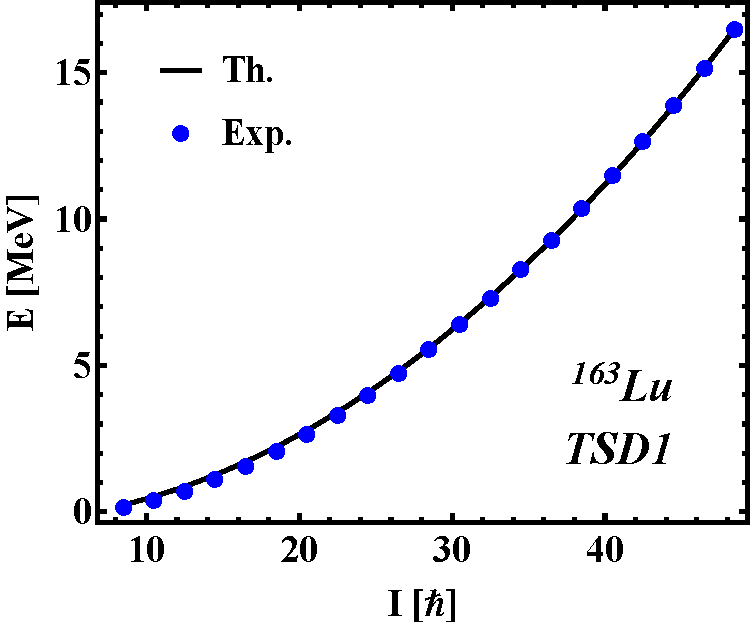
\includegraphics[scale=0.55]{figs/DoubleShift_TSD1.pdf}
\end{minipage}%
\begin{minipage}{.5\textwidth}
  \centering
 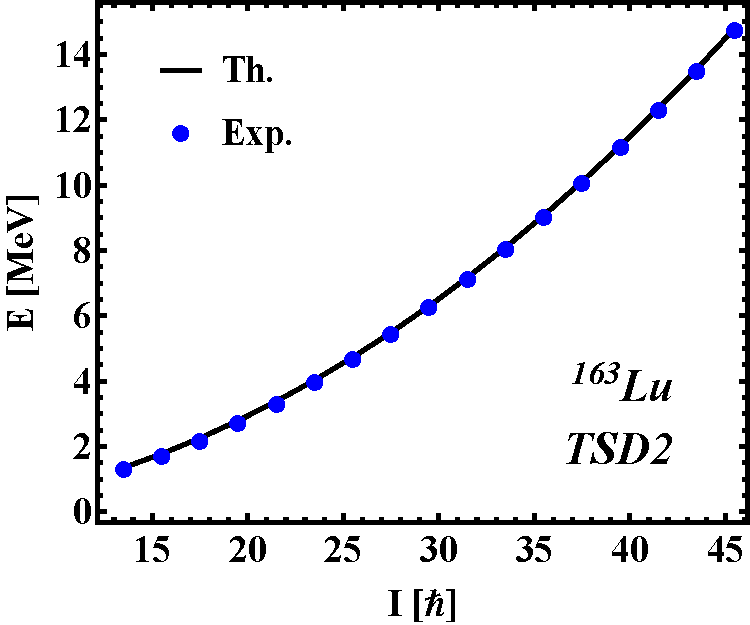
\includegraphics[scale=0.55]{figs/DoubleShift_TSD2.pdf}
\end{minipage}
\caption{Comparison between theoretical and experimental excitation energies for the first two wobbling bands in $^{163}$Lu within the \texttt{W2} model. The theoretical results are obtained with the parameters listed in Table \ref{parameter_set}. Experimental data is taken from \cite{reich2010nuclear}.}
\label{energies-tsd12}
\end{figure}

\begin{figure}
\centering
\begin{minipage}{.5\textwidth}
  \centering
  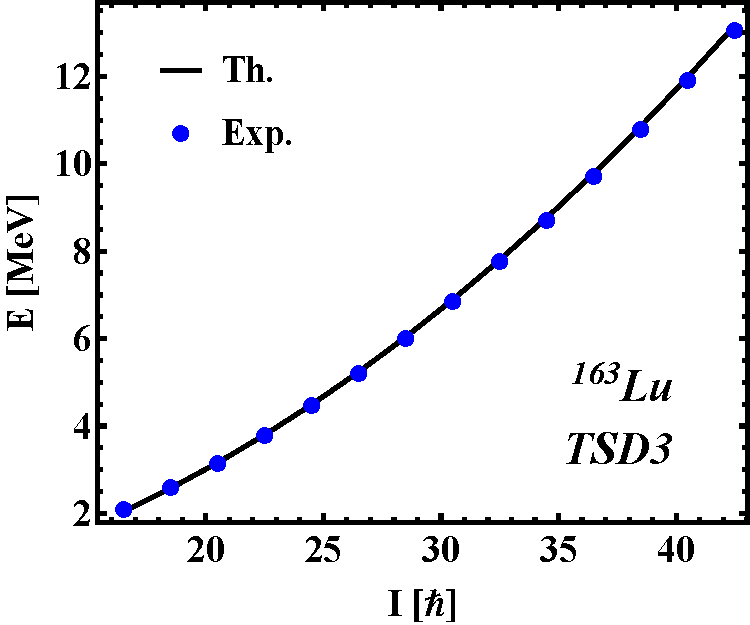
\includegraphics[scale=0.55]{figs/DoubleShift_TSD3.pdf}
\end{minipage}%
\begin{minipage}{.5\textwidth}
  \centering
 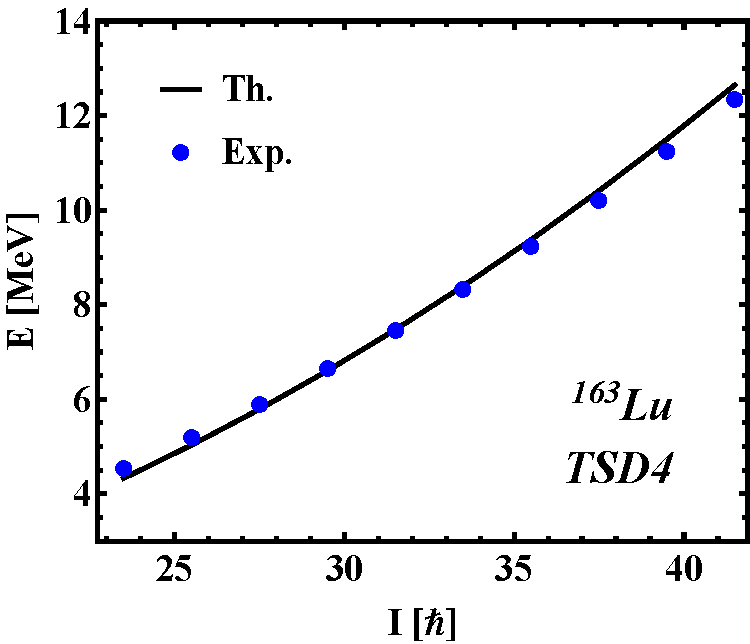
\includegraphics[scale=0.55]{figs/DoubleShift_TSD4.pdf}
\end{minipage}
\caption{Comparison between theoretical and experimental excitation energies for third and fourth wobbling bands in $^{163}$Lu within the \texttt{W2} model. The theoretical results are obtained with the parameters listed in Table \ref{parameter_set}. Experimental data is taken from \cite{reich2010nuclear}.}
    \label{energies-tsd34}
\end{figure}

Another noteworthy aspect of the current formalism is the fact that the difference $\delta_{42}=E_\text{TSD4}^I-E_\text{TSD2}^I$ for all the states has an a constant value $\delta_{42}=0.3\ \text{MeV}$. This suggests that the states of the same a.m. from $TSD_2$ and $TSD_4$ bands might emerge through the parity projection of a sole wave-function that does not have reflection symmetry. In the present case, this is caused by the fact that the wobbling frequency is parity independent. Consequently, these two bands indeed behave as a pair of parity partners, as defined in \cite{chasman1980incipient,raduta2006description,raduta2006simultaneous}.

% \subsection{Interpretation of the parameter set $\mathcal{P}$}
\subsection{\texorpdfstring{Interpretation of the parameter set $\mathcal{P}$}%
                               {Interpretation of the parameter set P}}

Performing the fitting procedure for the excitation energies of $^{163}$Lu results in the moments of inertia $\mathcal{I}_k$ given in Table \ref{parameter_set}, together with the single-particle potential strength $V$, and triaxiality parameter $\gamma$. Interpretation of their numerical values is mandatory in order to check whether the current formalism is valid or not.

Regarding the moments of inertia, it is clear that the axis of rotation for the energy ellipsoid is the 1-axis, as the largest MOI is $\mathcal{I}_1$, causing a maximal density distribution across this axis \cite{frauendorf2014transverse}. The MOI ordering is $\mathcal{I}_1>\mathcal{I}_2>\mathcal{I}_3$, and compared with the results of the previous work \texttt{W1}, the current 1-axis MOI is bigger than both $\mathcal{I}_1^\text{TSD1,2,3}=63.2$ and $\mathcal{I}_1^\text{TSD4}=67$ (data taken from Table 1 in Ref. \cite{raduta2020towards}). This is expected, since here, $TSD_4$ band is obtained by the coupling of a higher aligned $j$ particle, driving the system to an even larger deformation. One must remember that these are the \emph{effective} MOIs of the entire system, that is the triaxial-rotor + odd-particle. No spin dependence has been inferred for the MOIs, so a possible change in the MOIs ordering with the increase in spin $I$ cannot be studied within the current description. Furthermore, this formalism does not contain microscopic terms, so no presumptions on what causes the obtained MOI ordering can be stated. Although, by working with a quadrupole deformed mean-field, the moments of inertia of the triaxial core should be indeed consistent with the hydrodynamic model. For the sake of completeness, Figure \ref{hydro-mois} shows the evolution of a hydro-dynamical set of MOIs with respect to the triaxiality parameter $\gamma$.

\begin{figure}
\centering
\begin{minipage}{.5\textwidth}
  \centering
  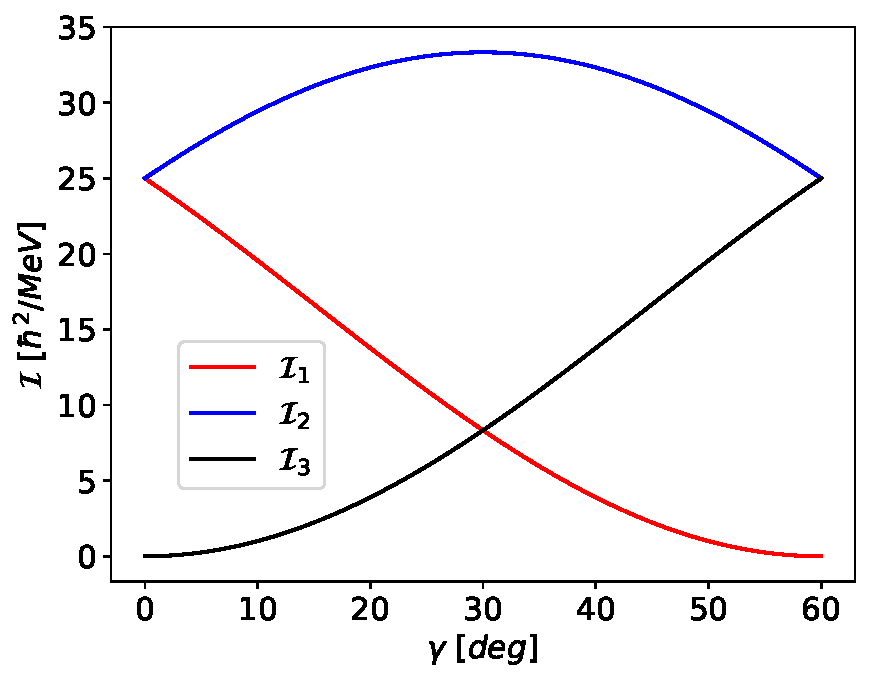
\includegraphics[scale=0.5]{figs/hydro_mois.pdf}
\end{minipage}%
\begin{minipage}{.5\textwidth}
  \centering
 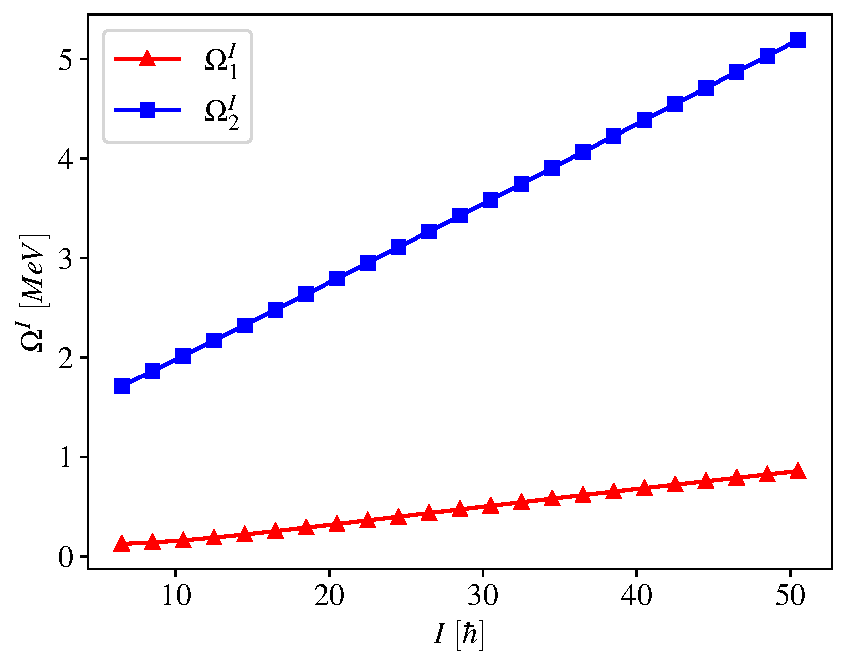
\includegraphics[scale=0.5]{figs/wobbling-frequencies.pdf}
\end{minipage}
\caption{Left-side: The hydrodynamic moments of inertia \cite{tanabe2006algebraic} as function of the triaxiality parameter $\gamma$, for the positive interval $\gamma\in[0^{\circ},60^{\circ}]$, evaluated for a scale factor $\mathcal{I}_0=25\ \text{MeV}^{-1}$. Right-side: The wobbling frequencies defined in Eq. \ref{wobbling-frequencies} as function of total angular momentum, evaluated with the parameter set $\mathcal{P}$ which was obtained through the fitting procedure.}
    \label{hydro-mois}
\end{figure}

Concerning the triaxiality parameter$\gamma$, it has a positive value $\gamma=22^\circ$. This is consistent with the microscopic descriptions based on cranking mechanism for the potential energy surface (PES) of $^{163}$Lu (discussion on PES was done in the previous sections). In fact, the agreement is quite good with the predicted deformed minima of $(\beta_2,\gamma)\approx(0.38,20^\circ)$ \cite{jensen2002wobbling,jensen2004coexisting}. Comparing the current \texttt{W2} model with already existing descriptions which take $\gamma$ to be fixed a-priori throughout the calculations (e.g., \cite{tanabe2006algebraic,tanabe2017stability}), here $\gamma$ is obtained through the fitting process in a self-consistent manner. Moreover, its value is slightly larger than the one obtained in \texttt{W1} formalism ($\gamma=17^\circ$). This might be due to the larger ratios $\mathcal{I}_1/\mathcal{I}_{2,3}$, which in the present case they appear to be bigger ($\mathcal{I}_1/\mathcal{I}_{2}\approx4.8$ for \texttt{W2}, compared to $\approx3.2$ in the previous approach \text{W1}).

Finally, the single-particle potential strength, which causes the odd-proton to move in the quadrupole deformed mean-field, has a value of $V=2.1\ \text{MeV}$. In \texttt{W1}, this parameter was $V^{\text{TSD1,2,3}}=3.1\ \text{MeV}$ and $V^\text{TSD4}=0.7\ \text{MeV}$. An explanation for its decrease in the present case might be due to the upward shift in the energy caused by the un-favored partner, or due to the energetic shift of the parity partner, indicating a quenching effect on the quadrupole deformation of the triaxial system. Nevertheless, the obtained value seems to be consistent with the previous calculations, The current $V$ beeing ckose to the average value of $V's$ in $W1$. Other interpretations \cite{tanabe2017stability} that were developed using a similar single-particle potential term in the Hamiltonian adopted values of around $V=1.6\ \text{MeV}$, however, that was for an isotope with smaller quadrupole deformation $\beta_2=0.18$. An interesting research devoted to the particle deformation in a single-$j$ shell model which was aimed at obtaining a realistic expression for the deformation parameter has been performed in \cite{shou2009coupling}. Therein, results for the potential strength of odd-$A$ nuclei with similar mass, but different quasiparticle configuration were numerically obtained. Adoption of an equivalent description for the odd-$j$ particle within \texttt{W2} could be adopted, and then compare results for a corresponding band configuration. This could be the motivating factor for future work made by the team. Concluding this subsection, the obtained values of $\mathcal{P}$ seem to not only describe the wobbling spectrum of $^{163}$Lu very well (see results in Figures \ref{energies-tsd12} and \ref{energies-tsd34}), but they are also consistent with the previous formalism \texttt{W1}, or even with other interpretations from the literature. 

\subsection{Stability of the wobbling region}

The expression for the classical energy function, which plays a crucial role in analyzing the nucleus' stability for a given rotational state, was presented in the previous section, with Eq. \ref{energy-function-minimal}. This will be used within the present numerical calculations to pinpoint the regions in the space where the minimal points of $\mathcal{H}$ arise. A special interest is devoted to the low-lying states from each of the four bands. Namely, for each band, a spin-state close to the band-head is chosen, then using the parameter set $\mathcal{P}$, a graphical representation in the $(\theta,\varphi)$-coordinate space is realized, and in each case, the extremal points with minimum character are identified. These graphical representations are shown in Figures \ref{contours-12} and \ref{contours-34}.

\begin{figure}
\centering
\begin{minipage}{.5\textwidth}
  \centering
  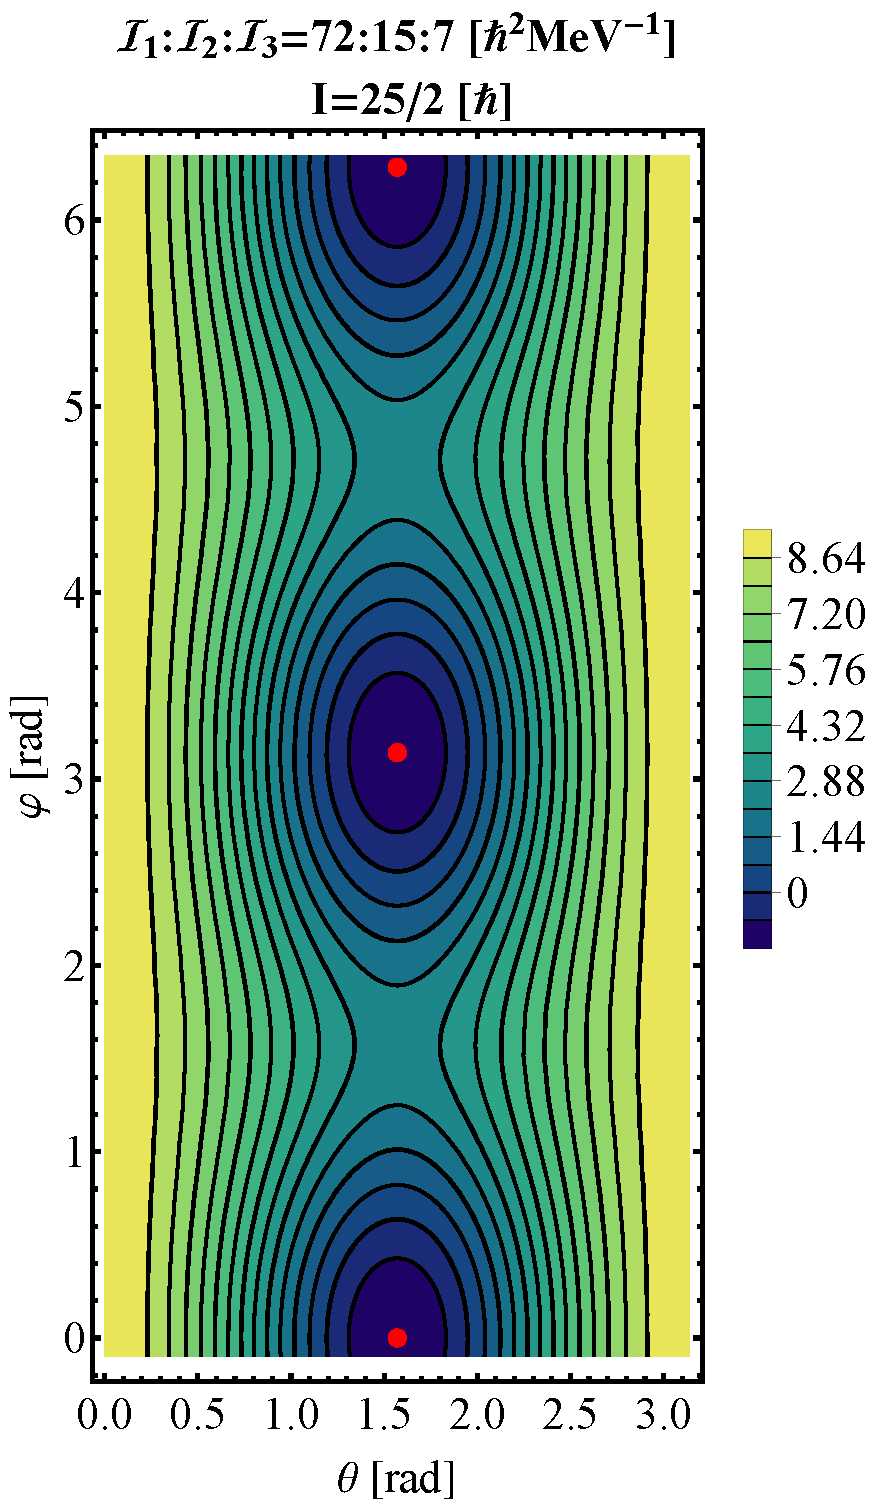
\includegraphics[scale=0.5]{figs/contour-tsd1.pdf}
\end{minipage}%
\begin{minipage}{.5\textwidth}
  \centering
 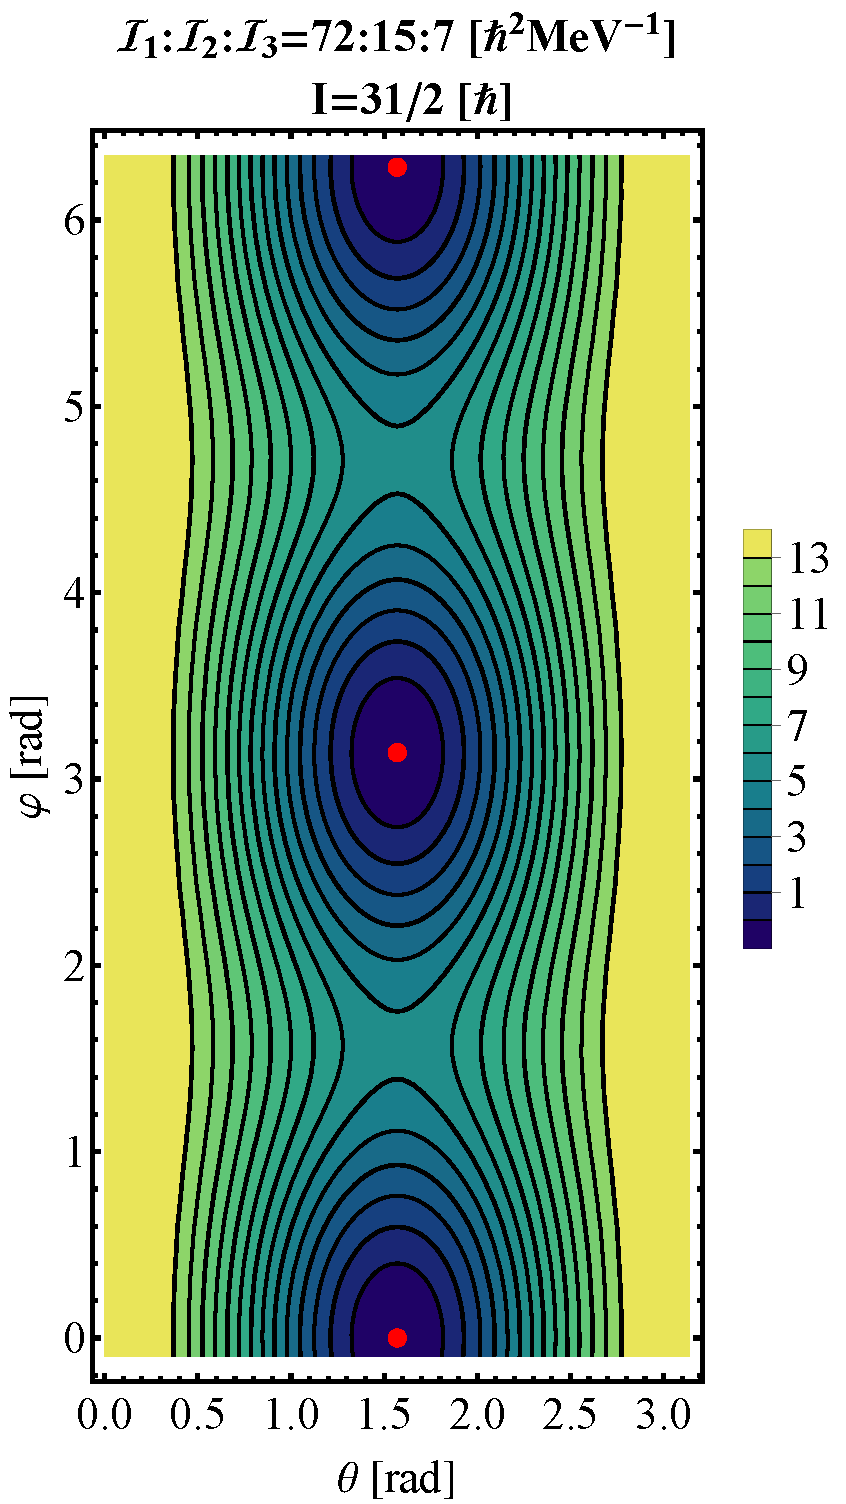
\includegraphics[scale=0.5]{figs/contour-tsd2.pdf}
\end{minipage}
\caption{Contour plots with the energy function $\mathcal{H}$ for a state in $TSD_1$ (left) and a state from $TSD_2$ (right). Calculations were performed with the numerical parameters obtained from the fitting procedure. The minimum points for $\mathcal{H}$ are marked by red dots, and they represent the regions in space where the nucleus has a stable wobbling character. The blue \emph{islands} also indicate a stable motion of the triaxial nucleus.}
    \label{contours-12}
\end{figure}

The four contour plots shown in Figures \ref{contours-12} and \ref{contours-34} have many similarities, suggesting common collective properties, but also differences caused by the fact that the minima have different depths. A common feature consists in that the equi-energy curves surround a sole minimum for low values in energy, but as the energy increases, the trajectories go around all minima, the lack of localization indicating unstable wobbling motion. The unstable regions might also relate to phase transitions, where the nucleus can undergo a major change in its rotational character. This aspect will be also discussed in the next subsection for the case of a 3-dimensional representation of the energy ellipsoid and the classical trajectories of the triaxial system.

\begin{figure}
\centering
\begin{minipage}{.5\textwidth}
  \centering
  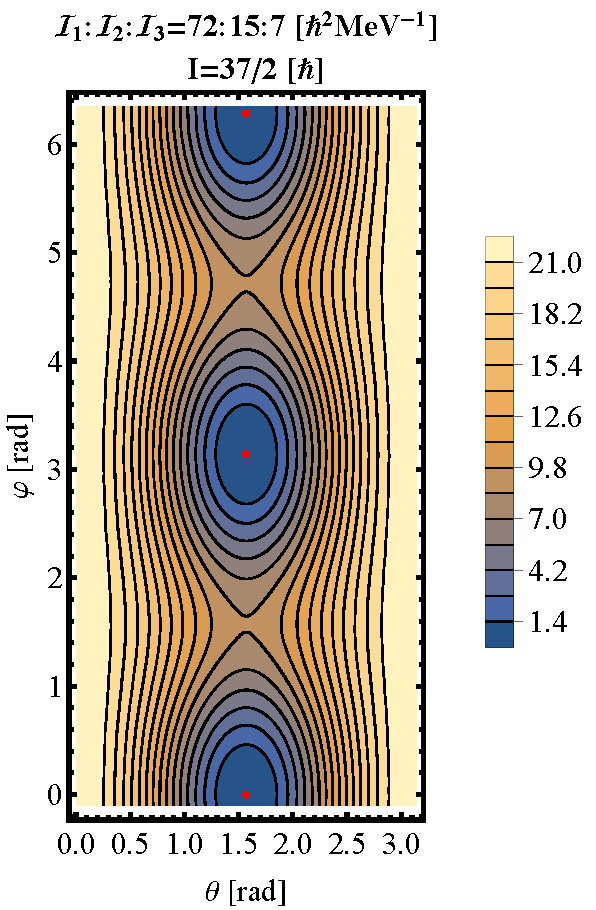
\includegraphics[scale=0.5]{figs/contour-tsd3.pdf}
\end{minipage}%
\begin{minipage}{.5\textwidth}
  \centering
 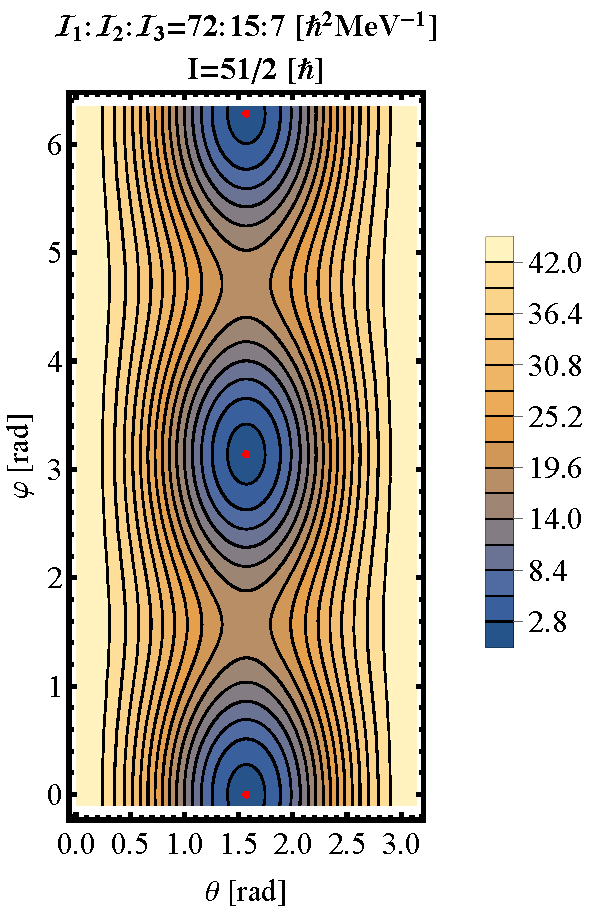
\includegraphics[scale=0.5]{figs/contour-tsd4.pdf}
\end{minipage}
\caption{Contour plots with the energy function $\mathcal{H}$ for a state in $TSD_3$ (left) and a state from $TSD_4$ (right). Calculations were performed with the numerical parameters obtained from the fitting procedure. The minimum points for $\mathcal{H}$ are marked by red dots, and they represent the regions in space where the nucleus has a stable wobbling character. The blue \emph{islands} also indicate a stable motion of the triaxial nucleus.}
    \label{contours-34}
\end{figure}

Regarding the minimum points (marked by red dots on the contour plots), their position remains unchanged for all four bands and any rotational state $I$, as long as the MOI's ordering stays the same. Remarkable is the fact that only with the obtained set of parameters (the current MOI ordering) it was possible to define contours with stable motion (marked by the blue regions). Indeed, if the two ratios $\mathcal{I}_1/\mathcal{I}_2$ and $\mathcal{I}_2/\mathcal{I}_3$ would have been smaller, a larger unstable region would prevail (with islands of maximal character), constraining thus the stable wobbling motion. This could indicate the fact that the single-particle term $T_\text{s.p.}$ from $\mathcal{H}$ actually \emph{prefers} a larger triaxiality in order to achieve a stable motion characterized by large deformation (see Eq. \ref{energyfunction-core-single-particle-subterms}).

An additional step consists in the analysis of the energy function, or more precisely to see its evolution in one of the minimal points concerning the angular momentum $I$. As it was already observed from the contour plots, the depth of the minima differ from one spin state to another, so it would be useful to have a quantitative view on that change. By fixing $\mathcal{H}$ in one of its critical points (e.g., the minimum $p_\text{min}(\theta,\varphi)=(\frac{\pi}{2},0)$), the angular momentum $I$ was varied within a large interval, and the evolution of $\mathcal{H}$ was evaluated. Graphical representation is shown in Figure \ref{energy-function-minimum-evolution}.

\begin{figure}
    \centering
    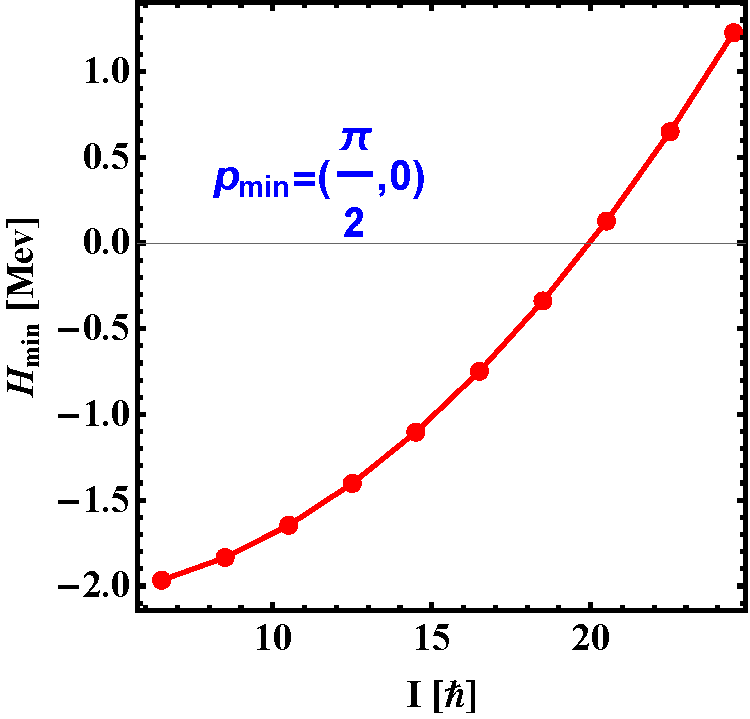
\includegraphics[scale=0.65]{figs/energy_function_minPoint_Evolution.pdf}
    \caption{The change in the minimum depth of $\mathcal{H}$, for the given parameter set $\mathcal{P}$, evaluated in the point $(\theta,\varphi)=(\frac{\pi}{2},0)$.}
    \label{energy-function-minimum-evolution}
\end{figure}

As it can be seen from Figure \ref{energy-function-minimum-evolution}, the classical energy $\mathcal{H}$ is an increasing function of angular momentum, which is to be expected, since the wobbling energies of the four bands increase with respect to the increase in spin. The negative values of $\mathcal{H}$ for low-lying wobbling states do not indicate that the nucleus has negative energy states since the rest of the nucleus' energy is also given by the single-particle energy $\epsilon_j$ terms and the phononic $\mathcal{F}_{n_{w_1}n_{w_2}}^I$ terms.

Another useful insight would be the study of the classical energy function $\mathcal{H}$ for the obtained parameter set, as a function of the polar angles $(\theta,\varphi)$. This can be achieved by choosing a minimum point, then keeping one of the polar coordinates fixed, and let the other one vary across its corresponding interval. For $^{163}$Lu, such a graphical representation was done for the point $p_\text{min}=\left(\frac{\pi}{2},0\right)$ (that is the bottom-most red dot from each of the four contour plots depicted in Figures \ref{contours-12} and \ref{contours-34}). Results can be seen in Figure \ref{energy-function-min-point-evolution}.

\begin{figure}
\centering
\begin{minipage}{.5\textwidth}
  \centering
  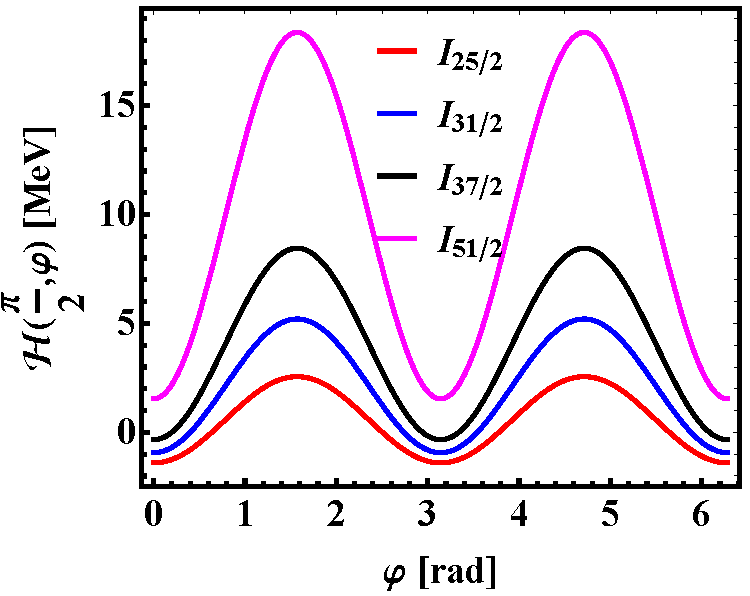
\includegraphics[scale=0.58]{figs/energyFunction_minTheta.pdf}
\end{minipage}%
\begin{minipage}{.5\textwidth}
  \centering
 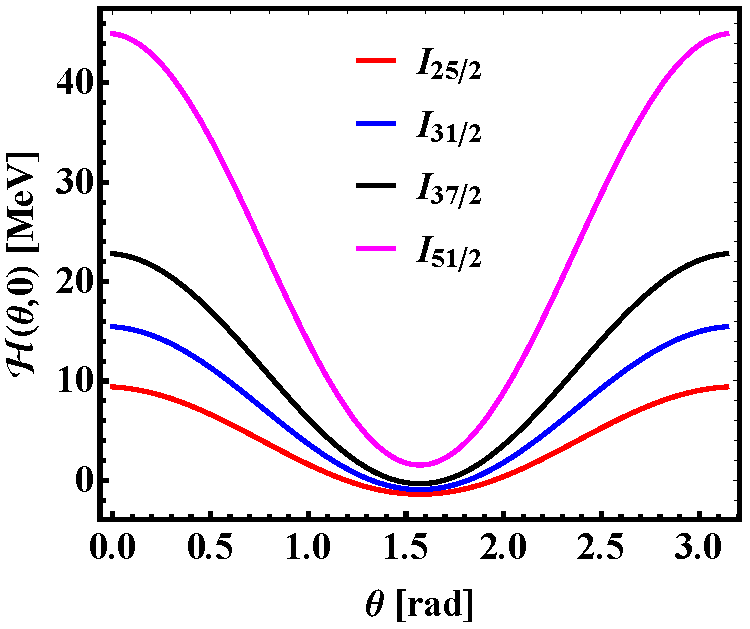
\includegraphics[scale=0.55]{figs/energyFunction_minVarphi.pdf}
\end{minipage}
\caption{The energy function $\mathcal{H}$, evaluated in one of its minimum points, as a function of the polar coordinates. One coordinate is fixed while the other one is varied within its interval of existence. For $\theta\in[0,\pi]$ and $\varphi\in[0,2\pi]$. The chosen minimum is $p_\text{min}=\left(\frac{\pi}{2},0\right)$. Each spin state corresponds to one of the four triaxial bands of $^{163}$Lu.}
    \label{energy-function-min-point-evolution}
\end{figure}

% \subsection{Comment on the wobbling nature of $^{163}$Lu}
\subsection{\texorpdfstring{Comment on the wobbling nature of $^{163}$Lu}%
                               {Comment on the wobbling nature of 163Lu}}

It is worthwhile discussing the results obtained regarding the wobbling spectrum of $^{163}$Lu. Indeed, using a fitting procedure that minimized the $\chi^2$ function, it was possible to find a parameter set $\mathcal{P}$ that when applied in the calculations for the excitation energies, an agreement with the experimental data is observed. However, in the current state, there is no clear evidence on whether the formalism \texttt{W2} predicts a TW or an LW behavior for the nucleus. According to \cite{frauendorf2014transverse}, the wobbling character is given by the coupling of the odd particle which aligns parallel (LW) or perpendicular (TW) to the axis with the largest MOI. But in order to see this within the measured data, an interpretation of the wobbling energy as it was defined in Eq. \ref{wobbling-energy-relative} must be performed. As such, according to the definition, one has to subtract an energy state within the first excited wobbling band (the one-wobbling-phonon band) from the average of its adjacent energies that belong to the yrast partner. In the present calculations, the first excited state is $TSD_3$, with its yrast partner being the band $TSD_2$. Following this procedure, both the experimental wobbling energies, as well as the theoretical ones were calculated according to the Eq. \ref{wobbling-energy-relative}. The obtained results are plotted in Figure \ref{wobbling-energies_th_exp}.

\begin{figure}
    \centering
    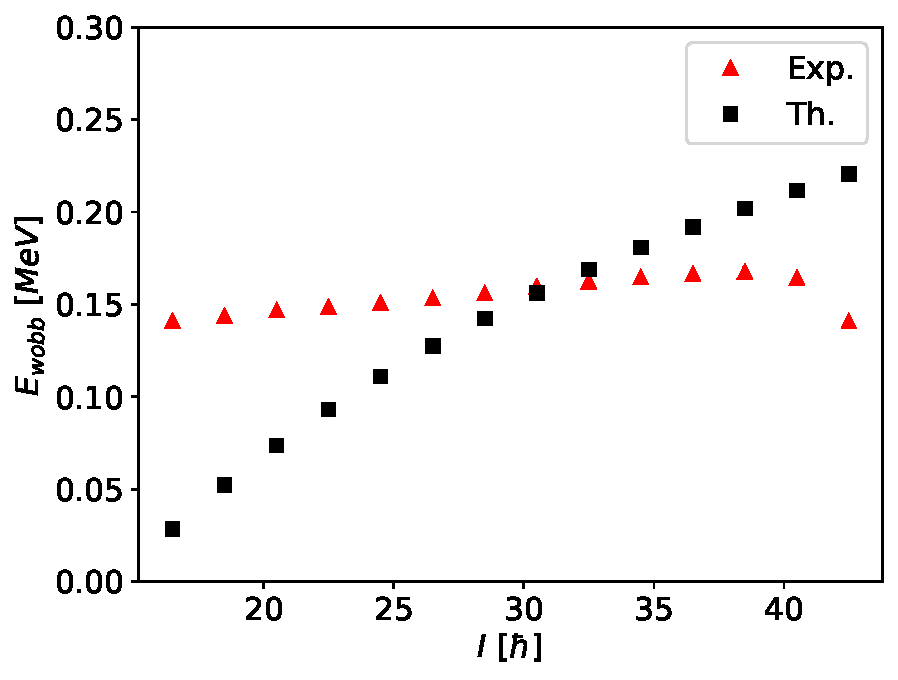
\includegraphics[scale=0.65]{figs/wobbling_energy_ThExp.pdf}
    \caption{The wobbling energies for $^{163}$Lu given as $E_\text{wob}=E_1(I)-\frac{1}{2}(E_0(I+1)+E_0(I-1))$. According to the current formalism, the sets of energies $E_1$ belong to $TSD_3$, while $E_0$ correspond to $TSD_2$. Experimental data is taken from \cite{reich2010nuclear}. Theoretical values were calculated with the parameter set $\mathcal{P}$.}
    \label{wobbling-energies_th_exp}
\end{figure}

From the behavior of $E_\text{wob}$ from Figure \ref{wobbling-energies_th_exp}, it can be seen that the theoretical wobbling spectrum is clearly an increasing function of angular momentum $I$, suggesting that $^{163}$Lu would have an LW character. This contrasts the current interpretation on which the wobbling energies are decreasing functions with the increase in spin. However, within those formalisms \cite{frauendorf2014transverse,frauendorf2018comment}, the wobbling energies are calculated with $TSD_2$ and $TSD_1$ instead, since the one-wobbling-phonon band is considered to be $TSD_2$, which is not consistent with the \texttt{W2} approach.

By contrast, analyzing the experimental data points from Figure \ref{wobbling-energies_th_exp}, a slight increase with spin can also be observed, suggesting as well that the coupling in $^{163}$Lu achieves an LW character. Indeed, from the lower limit of around $11/2\ \hbar$ and up to a spin of about $39/2\ \hbar$, the energy is increasing, then starts to decrease once $I\geq39/2\ \hbar$. The increasing behavior of the theoretical data also appears to be quenched in the high-spin limit, indicating that indeed, once the nucleus reaches high rotational states, a change in the wobbling regime might emerge, and the nucleus can transition from a wobbling regime (LW) to another (TW).

In a recent work \cite{nandi2020first}, an observation of two wobbling bands was made for $^{183}$Au. The bands are based on a positive $\pi(i_{13/2})$ and negative $\pi(h_{9/2})$ parity configuration, respectively. The remarking aspect of this research is that within a PRM model amended with the HFA (harmonic frozen alignment) approximation, it results that both bands have a transverse character (TW). However, they have different behavior with respect to the wobbling energies. Namely, this quantity increases (decreases) with spin for the positive (negative) parity configuration (see Figure 3 from \cite{nandi2020first}). According to the same study, the increasing trend of the positive parity band with spin has indeed a LW character, but it might be the \emph{initial part} of a TW band predicted by Frauendorf \cite{frauendorf2014transverse} for $^{163}$Lu, but never observed. This indicates that an increasing/decreasing behavior for $E_\text{wob}$ is not enough evidence for asserting a wobbling character on a triaxial nucleus (at least, not without some strong constraints on the coupling scheme between the core and the odd particle).

Concluding this comment on the wobbling nature for $^{163}$Lu, if the behavior of the wobbling energies with spin is the sole player in determining the wobbling character of a nucleus, then one could argue that indeed, based on the current results, $^{163}$Lu behaves as a longitudinal wobbler. On the other hand, considering the newly obtained results discussed in the previous paragraph, the evidence is not enough for making a clear assumption on which type of wobbling motion occurs.

\subsection{Classical trajectories - 3-dimensional representation}

The final step of the present work is to obtain an insight into the classical features of the triaxial nucleus in terms of its motion. As discussed already mentioned, the trajectories  are given by the intersection curves of the energy ellipsoid ($E$ given in Eq. \ref{energy-ellipsoid-cartesian}) and the angular momentum sphere ($I^2$ given in Eq. \ref{angular-momentum-sphere}). In the 3-dimensional space generated by the three components of the angular momentum vector $\vec{I}$, these intersection curves characterize the motion of the system, as each curve will be oriented along one of the three axes $x_k\ ,\ k=1,2,3$, suggesting a rotational motion (the precession of the total a.m.) around a particular direction preferred by the system.

The dependence of the classical trajectories on the angular momenta as well as on energies is thus analyzed with this model. Indeed, when the model Hamiltonian is diagonalized for a given $I$, a set of $2I+1$ energies are obtained. Therefore, it is justified to study the evolution of trajectories when the energy of the nucleus is increasing. The curves are represented as the manifold given by the intersection of the two constants of motion, that is $E$ and $I^2$. An example of such trajectories are depicted in Figures \ref{trajectories-12} and \ref{trajectories-34}.

\begin{figure}
    \centering
    % 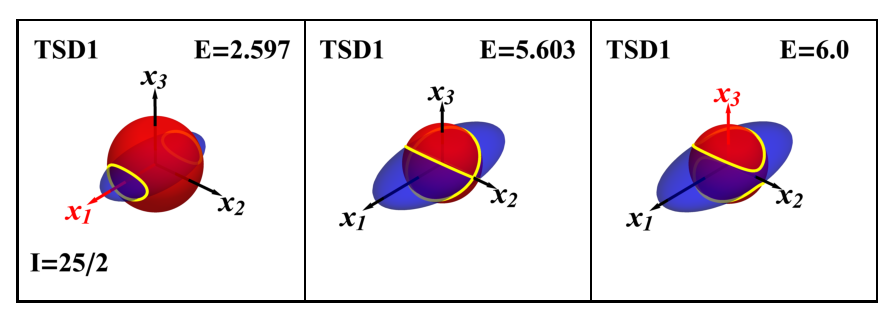
\includegraphics[width=0.8\textwidth]{figs/tsd1_spin1.eps}
    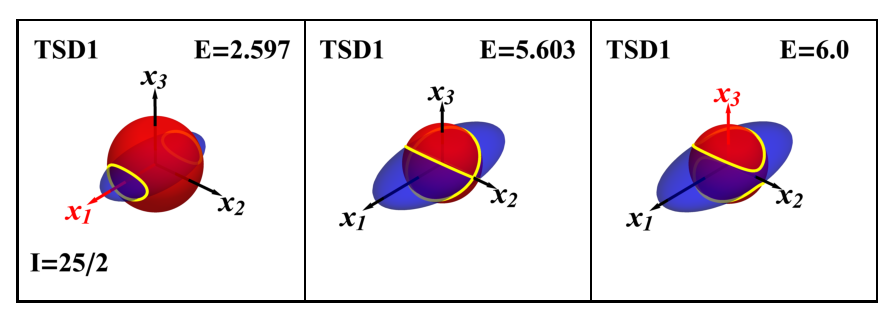
\includegraphics[scale=0.7]{figs/tsd1_spin1.eps}
    % 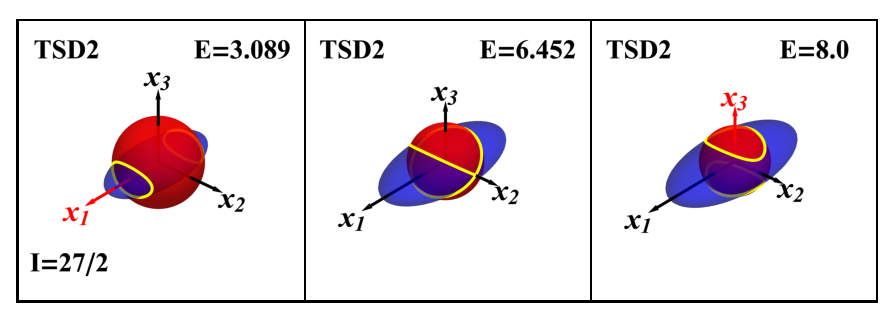
\includegraphics[width=0.8\textwidth]{figs/tsd2_spin1.eps}
    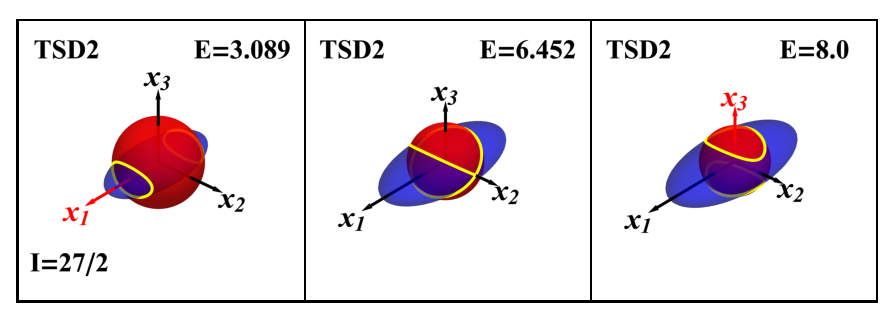
\includegraphics[scale=0.7]{figs/tsd2_spin1.eps}
    \caption{The nuclear trajectory of the system, for two spin states belonging to the first two wobbling bands in $^{163}$Lu. Intersection line marked by yellow color represents the actual orbits. Axis colored in red represents the direction along which the system rotates (it precesses). Left-most inset corresponds to the real excitation energy for that particular spin $I$.}
    \label{trajectories-12}
\end{figure}


\begin{figure}
    \centering
    % 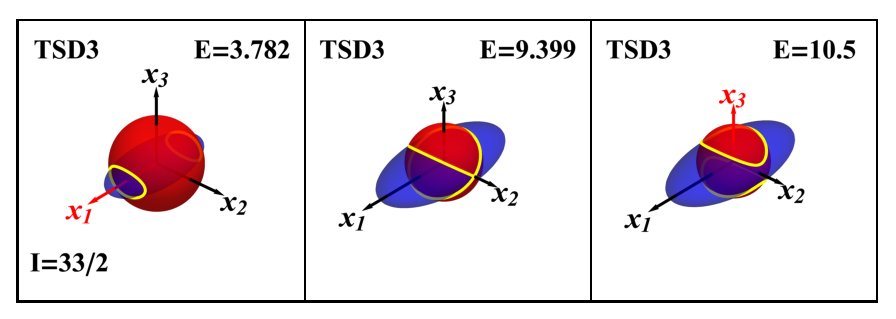
\includegraphics[width=0.8\textwidth]{figs/tsd3_spin1.eps}
    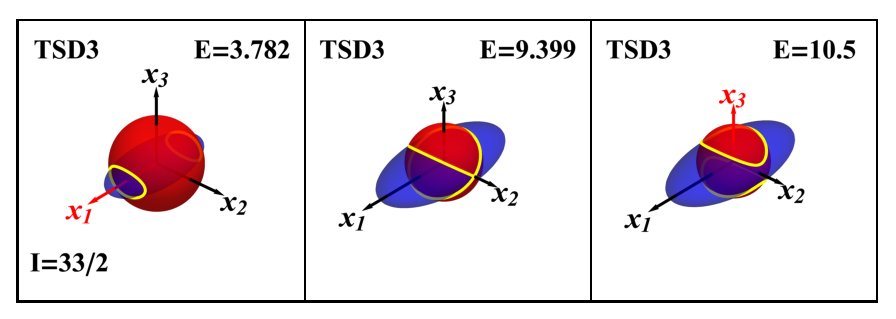
\includegraphics[scale=0.7]{figs/tsd3_spin1.eps}
    % 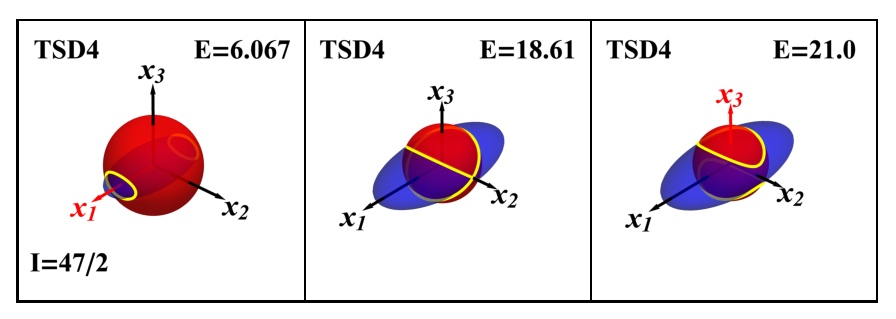
\includegraphics[width=0.8\textwidth]{figs/tsd4_spin1.eps}
    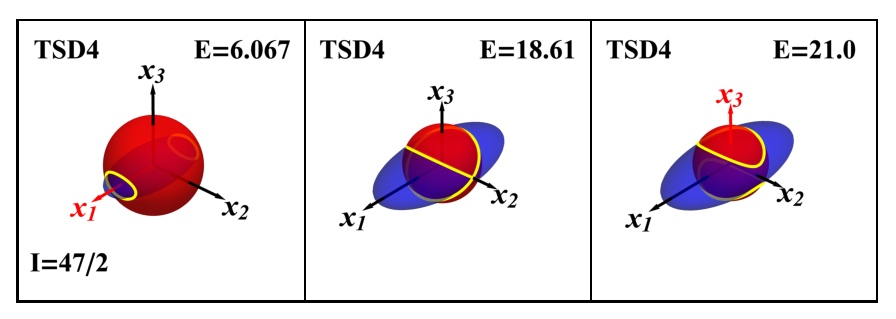
\includegraphics[scale=0.7]{figs/tsd4_spin1.eps}
    \caption{The nuclear trajectory of the system, for two spin states belonging to the third and fourth wobbling bands in $^{163}$Lu. Intersection line marked by yellow color represents the actual orbits. Axis colored in red represents the direction along which the system rotates (it precesses). Left-most inset corresponds to the real excitation energy for that particular spin $I$.}
    \label{trajectories-34}
\end{figure}

From Figures \ref{trajectories-12} and \ref{trajectories-34}, each row represents a rotational state within a band. A low-lying spin state was chosen from each band in particular as an example. The left inset within each row represents the real excitation energy for the state $I$ at which the energy ellipsoid is evaluated. It can be seen that two distinct (but symmetric) trajectories are observed along the 1-axis, for all four states. This suggests that the states of the triaxial nucleus are obtained from the rotation of the angular momentum along $x_1$. Indeed, for low energies, the rotation is pronounced along $x_1$- and $-x_1$-axis. As the energy of the nucleus increases, the two trajectories approach each other, which results in a tilted rotation axis corresponding to both curves. The tilted axis implies that the rotation axis is being misaligned, the rotational axis moving away from its \emph{equilibrium point}, marking the tilted-axis-rotation. Note that this  picture is fully consistent with the one described by Lawrie. Further increase in energy will result in the two trajectories intersect with each other. That particular point where the intersection between the two orbits occurs is marked in the middle inset from each figure. Consequently, the intersection of these two orbits marks an unstable motion within the system. Finally, when the energy increases even more, beyond that \emph{critical point}, one arrives again at two trajectories regime but with different rotation axis, which aligns closer to the $x_3$ axis. This case is shown in the right inset within each figure, where the axis $x_3$ is marked by red color, signaling the change in the rotation of the nucleus. However, it is worth noting that such energies are way too large for this phase transition to occur naturally for the studied spin-states. For example, in the case of $I_{25/2}\in TSD_1$, the energy at which $^{163}$Lu undergoes a phase transition with regards to the rotational mode is close to $5.6\ \text{MeV}$, but the real excitation energy which corresponds to this state is half in magnitude. Nevertheless, it is a remarkable fact that with the current model, a phase transition between rotational modes can be identified. A proper microscopic formalism based on this current approach might also provide a more detailed picture with regards to the allowed trajectories for the system.

\section{Conclusions \& Outlook}

The purpose of the present work was two-fold. On one hand, a detailed overview regarding the current experimental observations for wobbling motion in even-even and even-odd nuclei across several mass regions was made in the introductory part. This was accompanied by a brief mention of most of the theoretical methods that are used for the microscopic/macroscopic description of the wobbling phenomenon which occurs in triaxial nuclei. Also in the first part of the paper, a schematic analysis on the characteristics of the wobbling motion was made, which concerned the coupling scheme involved in a longitudinal/transverse wobbler. Therein, it was shown that depending on the alignment of the odd quasiparticle with the triaxial core, a certain wobbling regime will prevail. That concluded the introduction of this research work.

On the other hand, the second purpose of the current paper was to extend a previous model that described the $^{163}$Lu isotope within a re-interpretation of its four wobbling bands $TSD_{1,2,3,4}$. The previous model was denoted here with \texttt{W1}, and it introduced the concept of signature partners between the bands $TSD_1$ and $TSD_2$. One showed that the nucleus can be described as a particle that is moving in a quadrupole deformed mean field generated by the core. In \texttt{W1}, there was an $i_{13/2}$ particle involved in the particle-rotor-coupling for the description of the first three triaxial bands , and another nucleon with negative parity,i.e., the $\pi(h_{9/2})$ intruder, to describe the band $TSD_4$. Based on this established formalism a new approach was developed here as an extension, denoted throughout the paper by \texttt{W2}. The new approach is using the same numerical recipe in solving the Hamiltonian of the system, however, in the present case, a sole trial function is constructed to admit eigenstates with both positive and negative parity. Indeed, despite the fact that $TSD_4$ is of an opposite parity than the first three, all bands are described by coupling a unique single-particle, $i_{13/2}$, to the core states of positive parity for $TSD_{1,2,3}$ and core states of negative parity for $TSD_4$. The coupling schemes for the wobbling bands within \texttt{W2} were denoted by $C'_1, C'_2, C'_3$. From the quantal Hamiltonian specific to a Particle Rotor Model, a set of analytical expressions for the excitation energies of each band were obtained, by applying a Time-Dependent Variational Principle with the trial function carefully chosen so that it allows a mixture of both positive and negative parity states. The excitation energies comprise a term that represents the classical energy function, obtained as the average of the Hamiltonian with the trial wave-function. A second term has a phonon character, being composed of two wobbling frequencies that were obtained as solutions to a dispersion-like equation. 

A set of free parameters emerged, containing the three moments of inertia, the single-particle potential strength $V$, and the triaxiality parameter $\gamma$. They were obtained through a fitting procedure - all four bands were fitted with the same parameter set, unlike the previous approach in \texttt{W1}. The resulted set provides an impressive agreement with the existing experimental data concerning the wobbling spectrum of this isotope, deviations from the experimental energies being with a r.m.s. equal to $79\ \text{keV}$. An interpretation of the numerical values of the obtained parameters was done in Section 4, and indeed, the obtained values are consistent with other formalisms from the literature. An additional comment on the wobbling nature of $^{163}$Lu was performed, and a study of the wobbling energy behavior with spin showed that the increasing trend might indicate a longitudinal character. Furthermore, the study of the classical energy function was done in a polar coordinate system, obtaining the contour plots for spin states belonging to each band. The critical points from those contour maps indicate stability in terms of wobbling behavior. Unstable regions also emerge at high rotational energies. Lastly, by intersecting the angular momentum sphere  with the energy ellipsoid, the classical trajectories can be obtained. The results for these 3-dimensional representations are discussed at the end of Section 4. From the graphical representations, three situations for a given spin state of $^{163}$Lu might occur. i) At low energies, the rotation axis is either the 1-axis or the -1 axis, resulting in two trajectories along this axis. ii) At a particular energy (\emph{critical energy}) the two orbits get close to each other until they intersect, marking the point of unstable motion within the nucleus. iii) If the energy increases even more, then the triaxial nucleus performs a tilted-axis-rotation, where the rotational axis slowly moves away from $x_1$, and it approaches $x_3$, becoming misaligned. The change from each step to the other marks a phase transition, when the nucleus undergoes a transformation with regards to its rotational behavior, thereby, changing the wobbling regime. It is remarkable the fact that the current approach, which is treated in a semi-classical way, is able to predict the change in the wobbling regime in the same nucleus, this being of large interest in the nuclear community since evidence of such behavior was scarce.

Concluding the present work, the newly developed formalism proves to be a successful tool for accurately describing the wobbling spectrum of $^{163}$Lu, but also for providing insight for the rotational motion of the nuclear system with respect to its total spin.

\section*{Acknowledgments}
This work was supported by UEFISCU through the project PCE- 16/2021.

\appendix
\section{Appendix - Workflow Diagrams}
Here, the two models described in Section 2, namely the formalism $\texttt{W1}$ (see Section \ref{subsection:w1}) and \texttt{W2} (see Section \ref{subsection:w2}) are schematically represented, based on the discussions made for each of the two approaches. The \texttt{W1} mode corresponds to the work given in Refs. \cite{raduta2020approach,raduta2020towards}, and the \texttt{W2} corresponds to the formalism developed in the present paper. 

For the formalism \texttt{W1}, the diagram is shown in Figure \ref{w1-model-worfklow}, while for the newly developed approach \texttt{W2}, the diagram is shown in Figure \ref{w2-model-worfklow}.

%\subsection{The \texttt{W1} model}
\begin{figure}
    \centering
    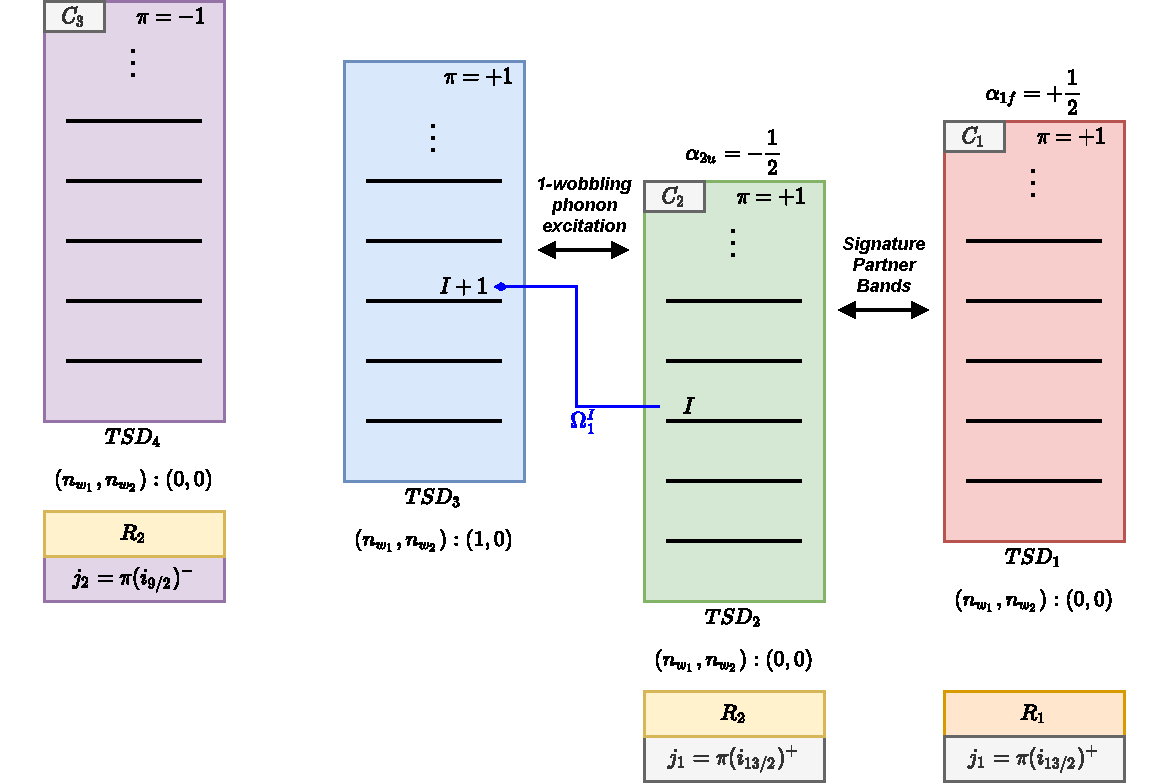
\includegraphics[scale=0.7]{figs/W1_model_approach.pdf}
    \caption{Illustrative depiction of the band structure adopted for $^{163}$Lu in the \texttt{W1} model. For each band, the wobbling phonon numbers are shown. The main features and linking properties between bands are represented with arrows. Bottom part shows the coupling schemes for each wobbling band, as described in text, namely $C_1$, $C_2$, $C_3$.}
    \label{w1-model-worfklow}
\end{figure}
%\subsection{The \texttt{W2} model}
\begin{figure}
   \centering
    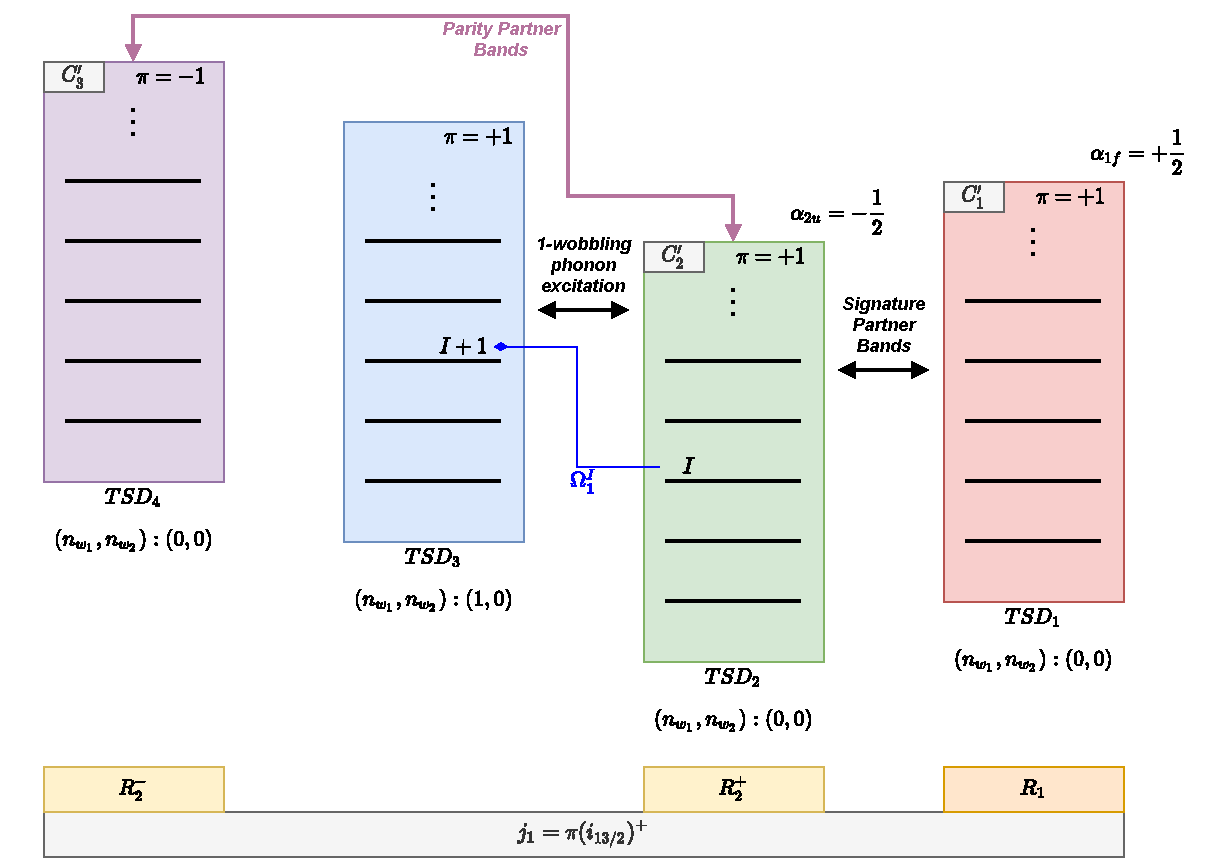
\includegraphics[scale=0.7]{figs/W2_model_approach.pdf}
    \caption{Illustrative depiction of the band structure adopted for $^{163}$Lu in the \texttt{W2} model. For each band, the wobbling phonon numbers are shown. The main features and linking properties between bands are represented with arrows. Bottom part shows the coupling schemes for each wobbling band, as described in text, namely $C'_1$, $C'_2$, $C'_3$.}
    \label{w2-model-worfklow}
\end{figure}
%%%%%%%%%%%%%%%%%%%%%%%%%%%%%%% TEXT  %%%%%%%%%%%%%%%%%%%%%%%%%%%%%%%%%%%%%%%%%
\newpage

\begin{thebibliography}{99}

\bibitem{moller2006global}
Peter M{\"o}ller, Ragnar Bengtsson, B~Gillis Carlsson, Peter Olivius, and
  Takatoshi Ichikawa.
\newblock Global calculations of ground-state axial shape asymmetry of nuclei.
\newblock {\em Physical review letters}, 97(16):162502, 2006.

\bibitem{moller2009heavy}
Peter M{\"o}ller, Arnold~J Sierk, Takatoshi Ichikawa, Akira Iwamoto, Ragnar
  Bengtsson, Henrik Uhrenholt, and Sven {\AA}berg.
\newblock Heavy-element fission barriers.
\newblock {\em Physical Review C}, 79(6):064304, 2009.

\bibitem{hamamoto1988triaxial}
I~Hamamoto and H~Sagawa.
\newblock Triaxial deformation in odd-z light rare-earth nuclei.
\newblock {\em Physics Letters B}, 201(4):415--419, 1988.

\bibitem{bengtsson1984signature}
R~Bengtsson, H~Frisk, FR~May, and JA~Pinston.
\newblock Signature inversion—a fingerprint of triaxiality.
\newblock {\em Nuclear Physics A}, 415(2):189--214, 1984.

\bibitem{stachel1982triaxiality}
J~Stachel, N~Kaffrell, E~Grosse, H~Emling, H~Folger, R~Kulessa, and D~Schwalm.
\newblock Triaxiality and its dynamics in 104ru investigated by multiple
  coulomb excitation.
\newblock {\em Nuclear Physics A}, 383(3):429--467, 1982.

\bibitem{frauendorf1997tilted}
Stefan Frauendorf and Jie Meng.
\newblock Tilted rotation of triaxial nuclei.
\newblock {\em Nuclear Physics A}, 617(2):131--147, 1997.

\bibitem{xiong2019nuclear}
BW~Xiong and YY~Wang.
\newblock Nuclear chiral doublet bands data tables.
\newblock {\em Atomic Data and Nuclear Data Tables}, 125:193--225, 2019.

\bibitem{raduta2016new}
AA~Raduta, Al~H Raduta, and CM~Petrache.
\newblock New type of chiral motion in even--even nuclei: the 138nd case.
\newblock {\em Journal of Physics G: Nuclear and Particle Physics}, 43(9):095107, 2016.

\bibitem{bohr1998nuclear}
Aage Bohr and Ben~R Mottelson.
\newblock {\em Nuclear structure}, volume~1.
\newblock World Scientific, 1998.

\bibitem{hagemann2003quantized}
Gudrun~B Hagemann and Ikuko Hamamoto.
\newblock Quantized wobbling in nuclei.
\newblock {\em Nuclear Physics News}, 13(3):20--24, 2003.

\bibitem{odegaard2001evidence}
SW~{\O}deg{\aa}rd, GB~Hagemann, DR~Jensen, M~Bergstr{\"o}m, B~Herskind,
  G~Sletten, S~T{\"o}rm{\"a}nen, JN~Wilson, PO~Tj{\o}m, I~Hamamoto, et~al.
\newblock Evidence for the wobbling mode in nuclei.
\newblock {\em Physical review letters}, 86(26):5866, 2001.

\bibitem{jensen2002evidence}
DR~Jensen, GB~Hagemann, I~Hamamoto, SW~{\O}deg{\aa}rd, B~Herskind, G~Sletten,
  JN~Wilson, K~Spohr, H~H{\"u}bel, P~Bringel, et~al.
\newblock Evidence for second-phonon nuclear wobbling.
\newblock {\em Physical review letters}, 89(14):142503, 2002.

\bibitem{jensen2002wobbling}
D~Ringk{\o}bing Jensen, GB~Hagemann, I~Hamamoto, SW~{\O}deg{\aa}rd,
  M~Bergstr{\"o}m, B~Herskind, G~Sletten, S~T{\"o}rm{\"a}nen, JN~Wilson,
  PO~Tj{\o}m, et~al.
\newblock Wobbling phonon excitations, coexisting with normal deformed
  structures in 163lu.
\newblock {\em Nuclear Physics A}, 703(1-2):3--44, 2002.

\bibitem{schnack1995superdeformed}
H~Schnack-Petersen, Ragnar Bengtsson, RA~Bark, P~Bosetti, A~Brockstedt,
  H~Carlsson, LP~Ekstr{\"o}m, GB~Hagemann, B~Herskind, F~Ingebretsen, et~al.
\newblock Superdeformed triaxial bands in 163,165 lu.
\newblock {\em Nuclear Physics A}, 594(2):175--202, 1995.

\bibitem{biswas2019longitudinal}
S~Biswas, R~Palit, S~Frauendorf, U~Garg, W~Li, GH~Bhat, JA~Sheikh, J~Sethi,
  S~Saha, Purnima Singh, et~al.
\newblock Longitudinal wobbling in 133 la.
\newblock {\em The European Physical Journal A}, 55(9):1--7, 2019.

\bibitem{matta2017transverse}
James~Till Matta.
\newblock Transverse wobbling in 135 pr.
\newblock In {\em Exotic Nuclear Excitations: The Transverse Wobbling Mode in
  135 Pr}, pages 77--93. Springer, 2017.

\bibitem{sensharma2019two}
N~Sensharma, U~Garg, S~Zhu, AD~Ayangeakaa, S~Frauendorf, W~Li, GH~Bhat,
  JA~Sheikh, MP~Carpenter, QB~Chen, et~al.
\newblock Two-phonon wobbling in 135pr.
\newblock {\em Physics Letters B}, 792:170--174, 2019.

\bibitem{chakraborty2020multiphonon}
S~Chakraborty, HP~Sharma, SS~Tiwary, C~Majumder, AK~Gupta, P~Banerjee,
  S~Ganguly, S~Rai, S~Kumar, A~Kumar, et~al.
\newblock Multiphonon longitudinal wobbling in 127xe.
\newblock {\em Physics Letters B}, 811:135854, 2020.

\bibitem{timar2019experimental}
J~Tim{\'a}r, QB~Chen, B~Kruzsicz, D~Sohler, I~Kuti, SQ~Zhang, J~Meng, P~Joshi,
  R~Wadsworth, K~Starosta, et~al.
\newblock Experimental evidence for transverse wobbling in pd 105.
\newblock {\em Physical review letters}, 122(6):062501, 2019.

\bibitem{nandi2020first}
S~Nandi, G~Mukherjee, QB~Chen, S~Frauendorf, R~Banik, Soumik Bhattacharya,
  Shabir Dar, S~Bhattacharyya, C~Bhattacharya, S~Chatterjee, et~al.
\newblock First observation of multiple transverse wobbling bands of different
  kinds in au 183.
\newblock {\em Physical Review Letters}, 125(13):132501, 2020.

\bibitem{sensharma2020longitudinal}
N~Sensharma, U~Garg, QB~Chen, S~Frauendorf, DP~Burdette, JL~Cozzi, KB~Howard,
  S~Zhu, MP~Carpenter, P~Copp, et~al.
\newblock Longitudinal wobbling motion in au 187.
\newblock {\em Physical review letters}, 124(5):052501, 2020.

\bibitem{guo2020risk}
S~Guo, XH~Zhou, CM~Petrache, EA~Lawrie, S~Mthembu, YD~Fang, HY~Wu, HL~Wang,
  HY~Meng, GS~Li, et~al.
\newblock Risk of misinterpretation of low-spin non-yrast bands as wobbling
  bands.
\newblock {\em arXiv preprint arXiv:2011.14354}, 2020.

\bibitem{hamilton2010super}
JH~Hamilton, SJ~Zhu, YX~Luo, AV~Ramayya, S~Frauendorf, JO~Rasmussen, JK~Hwang,
  SH~Liu, GM~Ter-Akopian, AV~Daniel, et~al.
\newblock Super deformation to maximum triaxiality in a= 100--112;
  superdeformation, chiral bands and wobbling motion.
\newblock {\em Nuclear Physics A}, 834(1-4):28c--31c, 2010.

\bibitem{petrache2019diversity}
CM~Petrache, PM~Walker, S~Guo, QB~Chen, S~Frauendorf, YX~Liu, RA~Wyss,
  D~Mengoni, YH~Qiang, A~Astier, et~al.
\newblock Diversity of shapes and rotations in the $\gamma$-soft 130ba nucleus:
  First observation of a t-band in the a= 130 mass region.
\newblock {\em Physics Letters B}, 795:241--247, 2019.

\bibitem{wang2020two}
YK~Wang, FQ~Chen, and PW~Zhao.
\newblock Two quasiparticle wobbling in the even-even nucleus 130ba.
\newblock {\em Physics Letters B}, 802:135246, 2020.

\bibitem{chen2019transverse}
QB~Chen, S~Frauendorf, and CM~Petrache.
\newblock Transverse wobbling in an even-even nucleus.
\newblock {\em Physical Review C}, 100(6):061301, 2019.

\bibitem{frauendorf2014transverse}
S~Frauendorf and F~D{\"o}nau.
\newblock Transverse wobbling: A collective mode in odd-a triaxial nuclei.
\newblock {\em Physical Review C}, 89(1):014322, 2014.

\bibitem{hamamoto2002wobbling}
Ikuko Hamamoto.
\newblock Wobbling excitations in odd-a nuclei with high-j aligned particles.
\newblock {\em Physical Review C}, 65(4):044305, 2002.

\bibitem{tanabe2006algebraic}
Kosai Tanabe and Kazuko Sugawara-Tanabe.
\newblock Algebraic description of triaxially deformed rotational bands in odd
  mass nuclei.
\newblock {\em Physical Review C}, 73(3):034305, 2006.

\bibitem{wen2015wobbling}
Shi Wen-Xian and Chen Qi-Bo.
\newblock Wobbling geometry in a simple triaxial rotor.
\newblock {\em Chinese Physics C}, 39(5):054105, 2015.

\bibitem{davydov1958rotational}
AS~Davydov and GF~Filippov.
\newblock Rotational states in even atomic nuclei.
\newblock {\em Nuclear Physics}, 8:237--249, 1958.

\bibitem{shimizu1995nuclear}
Yoshifumi~R Shimizu and Masayuki Matsuzaki.
\newblock Nuclear wobbling motion and electromagnetic transitions.
\newblock {\em Nuclear Physics A}, 588(3):559--596, 1995.

\bibitem{matsuzaki2002wobbling}
Masayuki Matsuzaki, Yoshifumi~R Shimizu, and Kenichi Matsuyanagi.
\newblock Wobbling motion in atomic nuclei with positive-$\gamma$ shapes.
\newblock {\em Physical Review C}, 65(4):041303, 2002.

\bibitem{matsuzaki2003dynamical}
Masayuki Matsuzaki, Yoshifumi~R Shimizu, and Kenichi Matsuyanagi.
\newblock Dynamical moments of inertia associated with wobbling motion in the
  triaxial superdeformed nucleus.
\newblock {\em The European Physical Journal A-Hadrons and Nuclei},
  20(1):189--190, 2003.

\bibitem{matsuzaki2004instability}
Masayuki Matsuzaki and Shin-Ichi Ohtsubo.
\newblock Instability of nuclear wobbling motion and tilted axis rotation.
\newblock {\em Physical Review C}, 69(6):064317, 2004.

\bibitem{matsuzaki2004nuclear}
Masayuki Matsuzaki, Yoshifumi~R Shimizu, and Kenichi Matsuyanagi.
\newblock Nuclear moments of inertia and wobbling motions in triaxial
  superdeformed nuclei.
\newblock {\em Physical Review C}, 69(3):034325, 2004.

\bibitem{shimizu2005high}
Yoshifumi~R Shimizu, Masayuki Matsuzaki, and Kenichi Matsuyanagi.
\newblock High-k precession modes: Axially symmetric limit of wobbling motion
  in the cranked random-phase approximation description.
\newblock {\em Physical Review C}, 72(1):014306, 2005.

\bibitem{shimizu2008parametrizations}
Yoshifumi~R Shimizu, Takuya Shoji, and Masayuki Matsuzaki.
\newblock Parametrizations of triaxial deformation and e 2 transitions of the
  wobbling band.
\newblock {\em Physical Review C}, 77(2):024319, 2008.

\bibitem{shoji2009microscopic}
Takuya Shoji and Yoshifumi~R Shimizu.
\newblock Microscopic calculation of the wobbling excitations employing the
  woods-saxon potential as a nuclear mean-field.
\newblock {\em Progress of theoretical physics}, 121(2):319--355, 2009.

\bibitem{chen2014collective}
QB~Chen, SQ~Zhang, PW~Zhao, and J~Meng.
\newblock Collective hamiltonian for wobbling modes.
\newblock {\em Physical Review C}, 90(4):044306, 2014.

\bibitem{chen2016wobbling}
QB~Chen, SQ~Zhang, J~Meng, et~al.
\newblock Wobbling motion in pr 135 within a collective hamiltonian.
\newblock {\em Physical Review C}, 94(5):054308, 2016.

\bibitem{mukhopadhyay2007chiral}
S~Mukhopadhyay, D~Almehed, U~Garg, S~Frauendorf, T~Li, PV~Madhusudhana Rao,
  X~Wang, SS~Ghugre, MP~Carpenter, S~Gros, et~al.
\newblock From chiral vibration to static chirality in nd 135.
\newblock {\em Physical review letters}, 99(17):172501, 2007.

\bibitem{qi2009chirality}
Bin Qi, SQ~Zhang, J~Meng, SY~Wang, and S~Frauendorf.
\newblock Chirality in odd-a nucleus 135nd in particle rotor model.
\newblock {\em Physics Letters B}, 675(2):175--180, 2009.

\bibitem{oi2000wobbling}
Makito Oi, Ahmad Ansari, Takatoshi Horibata, and Naoki Onishi.
\newblock Wobbling motion in the multi-bands crossing region.
\newblock {\em Physics Letters B}, 480(1-2):53--60, 2000.

\bibitem{raduta2017semiclassical}
AA~Raduta, R~Poenaru, and L~Gr Ixaru.
\newblock Semiclassical unified description of wobbling motion in even-even and
  even-odd nuclei.
\newblock {\em Physical Review C}, 96(5):054320, 2017.

\bibitem{raduta2020new}
AA~Raduta, CM~Raduta, and R~Poenaru.
\newblock A new boson approach for the wobbling motion in even--odd nuclei.
\newblock {\em Journal of Physics G: Nuclear and Particle Physics},
  48(1):015106, 2020.

\bibitem{tanabe1971triaxiality}
K~Tanabe and K~Sugawara-Tanabe.
\newblock Triaxiality in nuclear rotational states.
\newblock {\em Physics Letters B}, 34(7):575--578, 1971.

\bibitem{tanabe2008selection}
Kosai Tanabe and Kazuko Sugawara-Tanabe.
\newblock Selection rules for electromagnetic transitions in triaxially
  deformed odd-a nuclei.
\newblock {\em Physical Review C}, 77(6):064318, 2008.

\bibitem{shimada2018rotational}
Mitsuhiro Shimada, Yudai Fujioka, Shingo Tagami, and Yoshifumi~R Shimizu.
\newblock Rotational motion of triaxially deformed nuclei studied by the
  microscopic angular-momentum-projection method. i. nuclear wobbling motion.
\newblock {\em Physical Review C}, 97(2):024318, 2018.

\bibitem{hara1995projected}
Kenji Hara and Yang Sun.
\newblock Projected shell model and high-spin spectroscopy.
\newblock {\em International Journal of Modern Physics E}, 4(04):637--785,
  1995.

\bibitem{zhao2016configuration}
PW~Zhao, P~Ring, and J~Meng.
\newblock Configuration interaction in symmetry-conserving covariant density
  functional theory.
\newblock {\em Physical Review C}, 94(4):041301, 2016.

\bibitem{konieczka2018gamow}
M~Konieczka, Markus Kortelainen, and W~Satu{\l}a.
\newblock Gamow-teller response in the configuration space of a
  density-functional-theory--rooted no-core configuration-interaction model.
\newblock {\em Physical Review C}, 97(3):034310, 2018.

\bibitem{raduta2007semiclassical}
AA~Raduta, R~Budaca, and CM~Raduta.
\newblock Semiclassical description of a triaxial rigid rotor.
\newblock {\em Physical Review C}, 76(6):064309, 2007.

\bibitem{raduta2018wobbling}
AA~Raduta, R~Poenaru, and Al~H Raduta.
\newblock Wobbling motion in lu within a semi-classical framework.
\newblock {\em Journal of Physics G: Nuclear and Particle Physics},
  45(10):105104, 2018.

\bibitem{budaca2018tilted}
R~Budaca.
\newblock Tilted-axis wobbling in odd-mass nuclei.
\newblock {\em Physical Review C}, 97(2):024302, 2018.

\bibitem{raduta2020approach}
AA~Raduta, R~Poenaru, and CM~Raduta.
\newblock New approach for the wobbling motion in the even-odd isotopes lu 161,
  163, 165, 167.
\newblock {\em Physical Review C}, 101(1):014302, 2020.

\bibitem{raduta2020towards}
AA~Raduta, R~Poenaru, and CM~Raduta.
\newblock Towards a new semi-classical interpretation of the wobbling motion in
  163lu.
\newblock {\em Journal of Physics G: Nuclear and Particle Physics},
  47(2):025101, 2020.

\bibitem{bengtsson1990high}
Tord Bengtsson.
\newblock The high-spin structure of 158er: A theoretical study.
\newblock {\em Nuclear Physics A}, 512(1):124--148, 1990.

\bibitem{gorgen2004quadrupole}
A~G{\"o}rgen, RM~Clark, M~Cromaz, P~Fallon, GB~Hagemann, H~H{\"u}bel, IY~Lee,
  AO~Macchiavelli, G~Sletten, D~Ward, et~al.
\newblock Quadrupole moments of wobbling excitations in lu 163.
\newblock {\em Physical Review C}, 69(3):031301, 2004.

\bibitem{hagemann2005triaxiality}
GB~Hagemann.
\newblock Triaxiality and wobbling.
\newblock {\em Acta Physica Polonica B}, 36(4):1043, 2005.

\bibitem{jensen2004coexisting}
DR~Jensen, GB~Hagemann, I~Hamamoto, B~Herskind, G~Sletten, JN~Wilson,
  SW~{\O}deg{\aa}rd, K~Spohr, H~H{\"u}bel, P~Bringel, et~al.
\newblock Coexisting wobbling and quasiparticle excitations in the triaxial
  potential well of 163 lu.
\newblock {\em The European Physical Journal A-Hadrons and Nuclei},
  19(2):173--185, 2004.

\bibitem{tanabe2017stability}
Kosai Tanabe and Kazuko Sugawara-Tanabe.
\newblock Stability of the wobbling motion in an odd-mass nucleus and the
  analysis of pr 135.
\newblock {\em Physical Review C}, 95(6):064315, 2017.

\bibitem{frauendorf2018comment}
S~Frauendorf.
\newblock Comment on “stability of the wobbling motion in an odd-mass nucleus
  and the analysis of pr 135”.
\newblock {\em Physical Review C}, 97(6):069801, 2018.

\bibitem{tanabe2018reply}
Kosai Tanabe and Kazuko Sugawara-Tanabe.
\newblock Reply to “comment on ‘stability of the wobbling motion in an
  odd-mass nucleus and the analysis of pr 135’”.
\newblock {\em Physical Review C}, 97(6):069802, 2018.

\bibitem{sun1994varied}
Yang Sun, Shuxian Wen, et~al.
\newblock Varied signature splitting phenomena in odd proton nuclei.
\newblock {\em Physical Review C}, 50(5):2351, 1994.

\bibitem{khalaf11properties}
AM~Khalaf, Hayam Yassin, and Eman R~Abo Elyazeed.
\newblock Properties of signature partner superdeformed bands in mercury
  nuclei.
\newblock {\em Journal: JOURNAL OF ADVANCES IN PHYSICS}, 11(1), 2015.

\bibitem{uma2015deltai}
VS~Uma and Alpana Goel.
\newblock $\delta$i= 1 staggering in signature partner pairs of super-deformed
  rotational bands in the a= 190 mass region.
\newblock {\em The European Physical Journal Plus}, 130(6):1--6, 2015.

\bibitem{mittal2016signature}
HM~Mittal and Anshul Dadwal.
\newblock Signature partner pairs of superdeformed rotational bands in 192tl.
\newblock In {\em Proceedings of the DAE-BRNS Symp. on Nucl. Phys}, volume~61,
  page 134, 2016.

\bibitem{hamamoto1983intrinsic}
Ikuko Hamamoto and Ben Mottelson.
\newblock On the intrinsic spectra of rotating nuclei with tri-axial shape.
\newblock {\em Physics Letters B}, 127(5):281--285, 1983.

\bibitem{hamamoto1987rotational}
Ikuko Hamamoto.
\newblock Rotational motion of triaxial shape in unfavoured-signature states of
  odd-a nuclei.
\newblock {\em Physics Letters B}, 193(4):399--404, 1987.

\bibitem{hamamoto2016interplay}
Ikuko Hamamoto.
\newblock Interplay between one-particle and collective degrees of freedom in
  nuclei.
\newblock {\em Physica Scripta}, 91(2):023004, 2016.

\bibitem{torilov2004spectroscopy}
S~Torilov, S~Thummerer, W~Von~Oertzen, Tz~Kokalova, G~De~Angelis, HG~Bohlen,
  A~Tumino, M~Axiotis, E~Farnea, N~Marginean, et~al.
\newblock Spectroscopy of 40 ca and negative-parity bands.
\newblock {\em The European Physical Journal A-Hadrons and Nuclei},
  19(3):307--317, 2004.

\bibitem{debray2000alternating}
ME~Debray, MA~Cardona, D~Hojman, AJ~Kreiner, M~Davidson, J~Davidson, H~Somacal,
  G~Levinton, DR~Napoli, S~Lenzi, et~al.
\newblock Alternating parity bands in 87 218 fr.
\newblock {\em Physical Review C}, 62(2):024304, 2000.

\bibitem{radutaa2009csm}
AA~Radutaa and CM~Radutab.
\newblock The csm extension for the description of positive and negative parity
  bands in even-odd nuclei.
\newblock {\em arXiv preprint arXiv:0903.0076}, 2009.

\bibitem{raduta2011simultaneous}
AA~RADUTA and CM~Raduta.
\newblock Simultaneous description of positive and negative parity bands in
  even-even and even-odd nuclei.
\newblock {\em ANNALS OF THE UNIVERSITY OF CRAIOVA, PHYSICS}, 21(1):28--53,
  2011.

\bibitem{meyer1975collective}
J~Meyer-ter Vehn.
\newblock Collective model description of transitional odd-a nuclei:(i). the
  triaxial-rotor-plus-particle model.
\newblock {\em Nuclear Physics A}, 249(1):111--140, 1975.

\bibitem{wang2008description}
SY~Wang, SQ~Zhang, B~Qi, J~Peng, JM~Yao, J~Meng, et~al.
\newblock Description of $\pi$ g 9/2 $\nu$ h 11/2 doublet bands in rh 106.
\newblock {\em Physical Review C}, 77(3):034314, 2008.

\bibitem{peng2003description}
J~Peng, J~Meng, and SQ~Zhang.
\newblock Description of chiral doublets in a~ 130 nuclei and the possible
  chiral doublets in a~ 100 nuclei.
\newblock {\em Physical Review C}, 68(4):044324, 2003.

\bibitem{koike2004chiral}
T~Koike, K~Starosta, and I~Hamamoto.
\newblock Chiral bands, dynamical spontaneous symmetry breaking, and the
  selection rule for electromagnetic transitions in the chiral geometry.
\newblock {\em Physical review letters}, 93(17):172502, 2004.

\bibitem{wang2007doublet}
SY~Wang, SQ~Zhang, B~Qi, and J~Meng.
\newblock Doublet bands in cs 126 in the triaxial rotor model coupled with two
  quasiparticles.
\newblock {\em Physical Review C}, 75(2):024309, 2007.

\bibitem{reich2010nuclear}
CW~Reich and Balraj Singh.
\newblock Nuclear data sheets for a= 163.
\newblock {\em Nuclear Data Sheets}, 111(5):1211--1469, 2010.

\bibitem{chasman1980incipient}
RR~Chasman.
\newblock Incipient octupole deformation and parity doublets in the odd mass
  light actinides.
\newblock {\em Physics Letters B}, 96(1-2):7--10, 1980.

\bibitem{raduta2006description}
AA~Raduta, CM~Raduta, and Amand Faessler.
\newblock Description of positive and negative parity dipole bands within the
  extended coherent state model.
\newblock {\em Physics Letters B}, 635(2-3):80--84, 2006.

\bibitem{raduta2006simultaneous}
AA~Raduta, Al~H Raduta, and CM~Raduta.
\newblock Simultaneous description of four positive parity bands and four
  negative parity bands.
\newblock {\em Physical Review C}, 74(4):044312, 2006.

\bibitem{shou2009coupling}
Wang Shou-Yu, Qi~Bin, and Zhang Shuang-Quan.
\newblock Coupling parameter in the single-j shell model.
\newblock {\em Chinese Physics Letters}, 26(5):052102, 2009.

\bibitem{lawrie2020tilted}
EA~Lawrie, O~Shirinda, and CM~Petrache.
\newblock Tilted precession and wobbling in triaxial nuclei.
\newblock {\em Physical Review C}, 101(3):034306, 2020.

\end{thebibliography}


\end{document}
